\documentclass[11pt,oneside]{article}

\usepackage[a4paper,margin=27mm,headheight=15pt]{geometry}
\usepackage[T1]{fontenc}
\usepackage[utf8]{inputenc}
\IfFileExists{libertinus.sty}{\usepackage{libertinus}}{\usepackage{lmodern}}
\usepackage{microtype}
\usepackage{amsmath,amssymb,amsthm,mathtools,mathrsfs}
\usepackage{bm}
\usepackage{booktabs,longtable,array,tabularx}
\usepackage{graphicx}
\usepackage{pgfplots}
\usepackage{xcolor}
\usepackage{enumitem}
\usepackage{fancyhdr}
\usepackage{titlesec}
\usepackage{listings}
\usepackage{xurl}
\usepackage{hyperref}
\usepackage[nameinlink,noabbrev]{cleveref}

\definecolor{linkblue}{RGB}{25,75,135}
\definecolor{shadegray}{RGB}{246,247,249}
\definecolor{rulegray}{RGB}{195,201,208}
\pgfplotsset{compat=1.18}
\hypersetup{
  colorlinks=true,
  linkcolor=linkblue,
  citecolor=linkblue,
  urlcolor=linkblue,
  pdftitle={Fabius--Rvachev New Frontiers},
  pdfauthor={Research report for Vladimir Reshetnikov's ProveIt project},
  pdfsubject={Log-concavity, native orthogonal polynomials, Christoffel reconstruction, rational products for pi, Gauss quadrature, Pade approximation, and Legendre--Gaunt determinants},
  pdfkeywords={Fabius function, Rvachev up-function, Thue--Morse, orthogonal polynomials, Szego asymptotics, Christoffel function, Hankel determinants, pi, Legendre polynomials, Lambert W}
}

\pagestyle{fancy}
\fancyhf{}
\fancyhead[L]{\small Fabius--Rvachev new frontiers}
\fancyhead[R]{\small\nouppercase{\leftmark}}
\fancyfoot[C]{\thepage}
\renewcommand{\headrulewidth}{0.4pt}

\titleformat{\section}{\Large\bfseries}{\thesection}{0.7em}{}
\titleformat{\subsection}{\large\bfseries}{\thesubsection}{0.7em}{}
\titleformat{\subsubsection}{\normalsize\bfseries}{\thesubsubsection}{0.7em}{}
\setcounter{secnumdepth}{3}
\setcounter{tocdepth}{2}
\setlist[itemize]{leftmargin=2em,itemsep=0.25em,topsep=0.4em}
\setlist[enumerate]{leftmargin=2.3em,itemsep=0.25em,topsep=0.4em}

% Long unbreakable inline mathematics occasionally leaves a line with no legal
% break point.  A small emergency stretch lets TeX loosen such a line rather
% than let it protrude into the margin; it applies only to lines that would
% otherwise be overfull.
\setlength{\emergencystretch}{2em}

\newtheorem{theorem}{Theorem}[section]
\newtheorem{proposition}[theorem]{Proposition}
\newtheorem{lemma}[theorem]{Lemma}
\newtheorem{corollary}[theorem]{Corollary}
\newtheorem{conjecture}[theorem]{Conjecture}
\theoremstyle{definition}
\newtheorem{definition}[theorem]{Definition}
\newtheorem{algorithm}[theorem]{Algorithm}
\newtheorem{example}[theorem]{Example}
\theoremstyle{remark}
\newtheorem{remark}[theorem]{Remark}
\newtheorem{warning}[theorem]{Warning}

\newcommand{\R}{\mathbb R}
\newcommand{\C}{\mathbb C}
\newcommand{\Q}{\mathbb Q}
\newcommand{\N}{\mathbb N}
\newcommand{\Z}{\mathbb Z}
\newcommand{\Up}{\operatorname{up}}
\newcommand{\sinc}{\operatorname{sinc}}
\newcommand{\wt}{\operatorname{wt}_2}
\newcommand{\e}{\mathrm e}
\newcommand{\ii}{\mathrm i}
\newcommand{\dd}{\,\mathrm d}
\newcommand{\Li}{\operatorname{Li}}
\newcommand{\Var}{\operatorname{Var}}
\newcommand{\E}{\mathbb E}
\newcommand{\Prob}{\mathbb P}
\newcommand{\bigO}{\mathcal O}
\newcommand{\smallo}{o}
\newcommand{\supp}{\operatorname{supp}}
\newcommand{\sgn}{\operatorname{sgn}}
\newcommand{\lcm}{\operatorname{lcm}}
\newcommand{\vtwo}{v_2}
\newcommand{\qbinom}[3]{\genfrac{[}{]}{0pt}{}{#1}{#2}_{#3}}
\newcommand{\repo}{\nolinkurl{Analysis/FabiusFunction}}
\newcommand{\lean}[1]{%
  \ifmmode\text{\nolinkurl{#1}}\else\nolinkurl{#1}\fi}
\newcommand{\leanevaltwo}[1]{%
  \nolinkurl{integral_eval}\texttt{\textsubscript{2}}\nolinkurl{#1}}

\newenvironment{proofidea}{\par\smallskip\noindent\textit{Proof architecture.}\ }{\hfill$\square$\par\smallskip}
\newenvironment{boxedremark}{%
  \par\smallskip\noindent\begin{center}\begin{minipage}{0.94\textwidth}%
  \color{black}\hrule\vspace{0.6em}\small
}{%
  \vspace{0.6em}\hrule\end{minipage}\end{center}\smallskip
}

\lstdefinestyle{pseudo}{
  basicstyle=\ttfamily\small,
  backgroundcolor=\color{shadegray},
  frame=single,
  rulecolor=\color{rulegray},
  columns=fullflexible,
  keepspaces=true,
  showstringspaces=false,
  xleftmargin=0.7em,
  xrightmargin=0.7em,
  aboveskip=0.8em,
  belowskip=0.8em
}

% Document-specific support required by this report.
\graphicspath{{figures/}}
\allowdisplaybreaks[2]
\numberwithin{equation}{section}

\newenvironment{statusbox}[1]{%
  \par\smallskip\noindent\begin{center}\begin{minipage}{0.94\textwidth}%
  \hrule\vspace{0.55em}\noindent\textbf{#1}\par\smallskip
}{%
  \vspace{0.55em}\hrule\end{minipage}\end{center}\smallskip
}

\lstdefinestyle{pythonstyle}{
  language=Python,
  basicstyle=\ttfamily\footnotesize,
  backgroundcolor=\color{shadegray},
  frame=single,
  rulecolor=\color{rulegray},
  columns=fullflexible,
  keepspaces=true,
  showstringspaces=false,
  breaklines=true,
  xleftmargin=0.7em,
  xrightmargin=0.7em,
  aboveskip=0.8em,
  belowskip=0.8em
}

\newcommand{\eps}{\varepsilon}
\newcommand{\norm}[1]{\left\lVert#1\right\rVert}
\newcommand{\abs}[1]{\left\lvert#1\right\rvert}
\newcommand{\floor}[1]{\left\lfloor#1\right\rfloor}
\newcommand{\ceil}[1]{\left\lceil#1\right\rceil}
\renewcommand{\repo}{\nolinkurl{Analysis/FabiusFunction/docs}}
\newcommand{\commit}{\nolinkurl{b863b90ee74ec0405af2d67ad04c61824c3aea00}}

\title{\bfseries Fabius--Rvachev New Frontiers\\[0.45em]
\large Log-concavity, native orthogonal polynomials, Christoffel reconstruction,\\
rational products for $\pi$, Gauss--Pad\'e structure, and Legendre--Gaunt determinants}
\author{Research report for Vladimir Reshetnikov's \texttt{ProveIt} project}
\date{30 August 2026}

\begin{document}
\maketitle

\begin{abstract}
Let $F$ denote the bounded Fabius function and let $w=\Up$ be Rvachev's even
$C^\infty$ probability density supported on $[-1,1]$.  The current
\texttt{ProveIt} corpus already develops exact dyadic arithmetic, the
Thue--Morse and infinite-sinc descriptions, moment recurrences, Bell--Bernoulli
formulae, Lambert-$W$ endpoint asymptotics, polynomial synthesis by translates
of $\Up$, and Fourier--Legendre expansions.  This report audits that corpus and
then develops a partly overlapping layer around the intrinsic convex and
spectral geometry of the probability measure
\[
  \dd\mu(x)=\Up(x)\dd x.
\]

First, $\mu$ is an infinite convolution of centered uniform laws.  Closure of
log-concavity under convolution and weak limits therefore proves that $\Up$,
and hence $F$ on $[0,1]$, is log-concave.  Combining this with
$F'(x)=2F(2x)$ gives the new Tur\'an inequality
\[
  F(2x)^2\ge 2F(x)F(4x),\qquad 0<x\le\tfrac14.
\]
For $g_n=-\log F(2^{-n})$ this becomes the sharp discrete-curvature bound
$g_n-2g_{n-1}+g_{n-2}\ge\log2$.

Second, let $\pi_n$ be the monic orthogonal polynomials for $\mu$,
\[
 \pi_{n+1}(x)=x\pi_n(x)-\beta_n\pi_{n-1}(x).
\]
The known logarithmic-square endpoint law places $\mu$ in the Szeg\H{o} class.
Classical OPRL theory then yields
\[
 \beta_n\longrightarrow\frac14,
 \qquad
 \frac1n\sum_{\pi_n(\xi)=0}\delta_\xi
   \Longrightarrow \frac{\dd x}{\pi\sqrt{1-x^2}},
\]
together with strong norm, ratio, and determinant asymptotics.  The associated
Christoffel function reconstructs the bump pointwise:
\[
 \Up(x)=\lim_{N\to\infty}
 \frac{N\lambda_N(x)}{\pi\sqrt{1-x^2}},\qquad -1<x<1.
\]
Because every moment is rational, $\lambda_N(0)$ is rational; since
$\Up(0)=1$, this gives the canonical rational limit
\[
  N\lambda_N(0)\longrightarrow\pi.
\]

The strong Szeg\H{o} asymptotic at the symmetry point gives a second, more
surprising formula.  Every $\beta_n$ is rational, yet
\[
 \boxed{\displaystyle
  \pi=2\prod_{j=1}^{\infty}\frac{\beta_{2j}}{\beta_{2j-1}}.}
\]
The finite products are rational.  They are linked exactly to the Christoffel
approximants by a harmonic-mean identity.  The same Jacobi data generate the
Gauss rules and the diagonal Pad\'e approximants of the Cauchy transform.
Finally, the repository's exact Legendre coefficients give a finite
Legendre--Gaunt Gram matrix whose determinants recover the $\beta_n$; this
closes a new exact circuit from dyadic Fabius values through Wigner $3j$
coefficients to $\pi$ and back to $\Up$ in a single exact circuit.

A fully commented Python program in the archive computes exact initial data and
4,800-digit data through $\beta_{200}$.  It finds strict increase toward
$1/4$ throughout the tested range and strongly suggests
\[
 \frac14-\beta_n\sim\frac{2}{\pi}\frac{(\log_2n)^2}{n^2},
 \qquad
 \pi-2\prod_{j=1}^{M}\frac{\beta_{2j}}{\beta_{2j-1}}
 \sim\frac{(\log_2M)^2}{M^2}.
\]
These rate statements and monotonicity are recorded as conjectures, not as
proved consequences of the computations.
\end{abstract}

\begin{statusbox}{Evidence and novelty boundary}
The report is pinned to repository snapshot \commit.  The recursive TeX tree
under \repo{} was inspected together with its current coverage, audit, archive,
and frontier manifests.  Canonical consolidated sources and the newest
Legendre/Lagrange reports were close-read; generated tables and superseded
siblings were cross-checked through their manifests and targeted formula
searches.  That audit found pre-existing Nevai-limit, $J$-fraction, Hankel, and
Gauss--Pad\'e programs in the canonical representation frontier.  It found no
matching report-level result for the log-concavity of $\Up$, the rational
Christoffel limits and alternating Jacobi product for $\pi$, or the finite
Gaunt/Wigner entry expansion. The determinant change-of-basis, Jacobi
cross-ratio, and equivalent finite rational Gaunt-sum entry expansion are now
formalized downstream; the Wigner/$3j$ identification and its factorial closed
form are not. ``New'' therefore applies only to the
non-overlapping claims relative to this repository snapshot, not to the whole
package and not as a claim of worldwide priority.  Every imported fact, new
proof, standard external theorem, numerical observation, and conjecture is
marked according to its status.
\end{statusbox}

\begin{statusbox}{Important statements developed or assembled here}
\begin{enumerate}
\item $\Up$ and $F|_{[0,1]}$ are log-concave; hence a dyadic Tur\'an inequality,
      strong discrete convexity of $-\log F(2^{-n})$, and convexity of the
      inverse in logarithmic probability coordinates.
\item The native up-law Jacobi coefficients satisfy $\beta_n\to1/4$; zeros
      converge to the arcsine law; the moment Hankel determinants have a sharp
      capacity-scale asymptotic with an explicit Fabius--Szeg\H{o} constant.
\item Christoffel functions reconstruct $\Up$ from exact rational moment
      matrices, and $N\lambda_N(0)\to\pi$ through rational numbers.
\item $\pi=2\prod_{j\ge1}\beta_{2j}/\beta_{2j-1}$, with an exact harmonic-mean
      relation between its partial products and the Christoffel approximants.
\item The Cauchy transform has the Jacobi $J$-fraction whose convergents are
      exact Gauss--Pad\'e approximants, while the Fourier--Legendre coefficients
      produce the same Jacobi data through finite rational Gaunt matrices.
\end{enumerate}
\end{statusbox}

\tableofcontents
\clearpage

\section{Corpus audit and choice of frontier}
\label{sec:audit}

\subsection{Snapshot and source strata}
The branch moved while this investigation was in progress, so all statements
are deliberately pinned to \commit, whose commit time is 30 August 2026.  The
source tree is not a single paper.  It has several strata:
\begin{enumerate}
\item the current proof-backed exposition
\path{Fabius_Function_and_Rvachev_Up/Fabius_Function_and_Rvachev_Up.tex};
\item the current mathematical glossary and the non-elementarity report;
\item vendored source papers, especially Arias de Reyna's 2017 analytic and
      arithmetic papers;
\item a consolidated semi-formalized frontier volume and thematic drafts on
      asymptotics, inverse functions, $q$-calculus, interpolation, integral
      transforms, spectral arithmetic, and representation theory;
\item recent Legendre and Lagrange closed-loop reports, including
      \path{legendre_rvachev_closed_loop.tex} and
      \path{legendre_rvachev_self_reconstruction.tex};
\item an archive of superseded expositions and early calculations; and
\item generated TeX tables that are inputs to larger reports rather than
      independent mathematical narratives.
\end{enumerate}
The coverage and audit documents are essential because the archive contains
near-duplicates with different correction levels.  Treating every archived
copy as independent would overcount evidence and, more seriously, could revive
claims explicitly corrected in the canonical exposition.

\subsection{What the corpus already contains}
The following list is a compressed dependency map, not a substitute for the
repository's much longer crosswalk.
\begin{itemize}
\item The bounded CDF $F$, the signed/global variants, the even bump $\Up$, the
      refinement and differential equations, support, smoothness, endpoint
      flatness, and partition-of-unity identities.
\item The weighted-uniform random series, finite convolutions, Fourier and MGF
      products, the Thue--Morse product, Poisson summation, and exact dyadic
      values.
\item Rational moments and their triangular recurrence, cumulants expressed by
      Bernoulli numbers, moments expressed by complete Bell polynomials, and
      positive moment Hankel matrices.
\item Sharp Fourier decay and log-periodic dyadic-shell structure, together
      with the small-argument endpoint law and its Lambert-$W$ inversion.
\item $q$-Pochhammer and Gaussian-binomial identities, geometric Richardson
      filters, and several exact finite interpolation/sampling mechanisms.
\item Fourier--Legendre expansions of $\Up$, finite synthesis of polynomials by
      shifted copies of $\Up$, and the resulting blockwise Legendre--Rvachev
      self-reconstruction.
\item Native orthogonal-polynomial data: exact moments and positive Hankel
      matrices, together with an all-degree exact rational layer for Hankel
      determinants, monic polynomial coefficients, norms, zero diagonal,
      positive Jacobi subdiagonals, orthogonality, determinant cross-ratio, and
      the centered recurrence; the separately evaluated low-degree table has
      the formal/report boundary stated in Section~\ref{sec:native-op}.
\item The moment Laurent series and a renormalization identity for the Cauchy
      transform.
\end{itemize}
The last two bullets are where this report begins, but the original novelty
screen was too broad.  At the pinned checkpoint the canonical representation
frontier already discussed the Nevai limit, the native J-fraction, and the
Gauss--Pad\'e program.  Those strands are therefore inherited overlap, not
evidence of absence from the corpus.  The report remains useful as a combined
treatment of log-concavity and the Fabius Tur\'an inequality, Christoffel
reconstruction, the rational product limits for \(\pi\), and the finite
Legendre--Gaunt bridge.  Its novelty language is repository-relative and must
be read subject to this corrected crosswalk.

\subsection{Why this direction avoids duplication}
The recent Legendre reports solve a different closure problem.  They begin
with an exact expansion of $\Up$ in the \emph{classical} Legendre basis and
replace each Legendre polynomial by a finite train of translated up-functions.
Here we instead orthogonalize polynomials against the \emph{native measure}
$\Up(x)\dd x$.  The resulting Jacobi matrix is an invariant of the probability
law itself.  It remembers all rational moments, controls Gaussian quadrature
and Pad\'e approximation, and has a universal large-degree limit fixed by the
support.  The two viewpoints meet only later, through the finite Gaunt matrix
of \cref{sec:legendre-gaunt}.

\begin{table}[htbp]
\centering
\caption{Claim-status summary.  ``Repository baseline'' means imported from
\commit; ``standard theorem'' means a classical external result whose
hypotheses are verified here.}
\label{tab:status}
\begin{tabularx}{\textwidth}{@{}p{0.29\textwidth}p{0.20\textwidth}X@{}}
\toprule
Statement & Status & Main input \\
\midrule
Uniform-series law, rational moments, endpoint log-square law
 & Repository baseline & Canonical exposition and formal moment modules \\
$\Up$ and $F$ are log-concave
 & New proof here & Convolution/weak-limit closure of log-concavity \\
Dyadic Tur\'an inequality and action curvature
 & New theorem here & Log-concavity plus $F'(x)=2F(2x)$ \\
$\beta_n\to1/4$, arcsine zeros
 & Overlap / application here & Canonical frontier; Rakhmanov/regular OPRL theory \\
Fabius--Szeg\H{o} norm constant
 & New application here & Strong Szeg\H{o} norm asymptotics \\
Christoffel reconstruction of $\Up$
 & New application here & M\'at\'e--Nevai--Totik/Totik asymptotics \\
Rational limits to $\pi$
 & New corollary here & $\Up(0)=1$ and rational moments \\
Alternating Jacobi product for $\pi$
 & New theorem here & Strong Szeg\H{o} center asymptotic \\
Gauss--Pad\'e package
 & Inherited overlap & Canonical frontier; classical Markov/Stieltjes theory \\
Legendre Gram determinant, executable rational data, and Jacobi cross-ratio
 & Exact Lean counterpart & \path{FabiusLegendreHankelDeterminant.lean};
   \path{FabiusLegendreRationalGram.lean};
   \path{FabiusLegendreRationalGramValues.lean} \\
Finite Gaunt integral, product linearization, and rational Gram-entry sum
 & Exact Lean counterpart & \path{LegendreGaunt.lean};
   \path{FabiusLegendreGaunt.lean} \\
Wigner $3j$ identification and factorial closed form
 & Report-level formula & Not represented in the current Lean API \\
Monotone $\beta_n$, precise log-square rate
 & Conjectural & Exact checks and 4,800-digit computation through $n=200$ \\
\bottomrule
\end{tabularx}
\end{table}

\section{Repository baseline and notation}
\label{sec:baseline}

\subsection{The Fabius and up laws}
Let $U_0,U_1,\ldots$ be independent uniform random variables on $[0,1]$, and
put
\begin{equation}
 X=\sum_{n=0}^{\infty}\frac{U_n}{2^{n+1}}.
 \label{eq:X-random}
\end{equation}
The bounded Fabius function is the distribution function
\begin{equation}
 F(x)=\Pr[X\le x].
 \label{eq:F-cdf}
\end{equation}
It is supported probabilistically on $[0,1]$, is strictly increasing there,
and obeys
\begin{equation}
 F'(x)=2F(2x),\qquad 0\le x\le\tfrac12,
 \label{eq:F-differential}
\end{equation}
with the usual reflected form on the other half.  Rvachev's bump is
\begin{equation}
 \Up(y)=F(1-\abs y),\qquad \abs y\le1,
 \label{eq:up-fold}
\end{equation}
and vanishes outside $[-1,1]$.  It is even, $C^\infty$, positive on
$(-1,1)$, flat at the endpoints, and normalized by
\begin{equation}
 \int_{-1}^{1}\Up(x)\dd x=1,
 \qquad \Up(0)=1.
 \label{eq:up-normalization}
\end{equation}

The centered random variable
\begin{equation}
 Y=2X-1=\sum_{n=0}^{\infty}2^{-n}\left(U_n-\tfrac12\right)
 \label{eq:Y-random}
\end{equation}
has density $\Up$.  Indeed, the density of $X$ is $F'(x)$; for $-1<y<0$,
\[
 \frac12F'\!\left(\frac{y+1}{2}\right)=F(y+1)=\Up(y),
\]
and symmetry gives the positive half.  Thus throughout the report
\begin{equation}
 \dd\mu(x)=\Up(x)\dd x
 \label{eq:mu-def}
\end{equation}
is both a compactly supported probability measure and an infinite convolution
of centered uniforms.

\subsection{MGF, cumulants, and rational moments}
The moment-generating function of $Y$ is the entire product
\begin{equation}
 M(z)=\int_{-1}^{1}\e^{zx}\dd\mu(x)
 =\prod_{j=1}^{\infty}\frac{\sinh(z/2^j)}{z/2^j}.
 \label{eq:mgf-product}
\end{equation}
Writing
\[
 \log M(z)=\sum_{r\ge1}\kappa_r\frac{z^r}{r!},
\]
all odd cumulants vanish and
\begin{equation}
 \kappa_{2r}=\frac{2^{2r-1}B_{2r}}{r(2^{2r}-1)}.
 \label{eq:cumulants}
\end{equation}
Consequently every moment is rational and can be written as a complete Bell
polynomial in the Bernoulli cumulants.  For the even moments
\begin{equation}
 c_n=m_{2n}=\int_{-1}^{1}x^{2n}\Up(x)\dd x,
 \qquad m_{2n+1}=0,
 \label{eq:moments}
\end{equation}
the particularly efficient triangular recurrence is
\begin{equation}
 (2n+1)(2^{2n}-1)c_n
 =\sum_{j=0}^{n-1}\binom{2n+1}{2j}c_j,
 \qquad c_0=1.
 \label{eq:moment-recurrence}
\end{equation}
The first values are
\begin{equation}
 c_0=1,
 \qquad c_1=\frac19,
 \qquad c_2=\frac{19}{675},
 \qquad c_3=\frac{583}{59535}.
 \label{eq:first-moments}
\end{equation}

\subsection{Endpoint law}
The sharp asymptotic program in the repository implies, in its simplest
invariant form,
\begin{equation}
 -\log F(x)\sim\frac{\log^2(1/x)}{2\log2}
 \qquad (x\downarrow0).
 \label{eq:endpoint-log-square}
\end{equation}
Therefore
\begin{equation}
 -\log\Up(1-\eps)\sim\frac{\log^2(1/\eps)}{2\log2}
 \qquad (\eps\downarrow0),
 \label{eq:up-endpoint-log-square}
\end{equation}
with the symmetric law at $-1$.  More refined repository formulae introduce a
Lambert-$W$ saddle coordinate and dyadic log-periodic corrections.  For the
spectral results below, the leading logarithmic-square envelope is enough.

\section{A new log-concavity theorem}
\label{sec:logconcavity}

\subsection{Infinite uniform convolution}
For $n\ge0$, let $\nu_n$ be the uniform probability law on
\[
 I_n=[-2^{-n-1},2^{-n-1}].
\]
Then \cref{eq:Y-random} says
\begin{equation}
 \mu=\nu_0*\nu_1*\nu_2*\cdots
 \label{eq:infinite-convolution}
\end{equation}
in the sense of weak convergence of the finite convolutions.

\begin{theorem}[Log-concavity of the up law]
\label{thm:up-logconcave}
The probability measure $\mu$ is log-concave.  Its continuous density
$\Up$ is log-concave on $\R$ in the extended sense, and strictly positive on
$(-1,1)$.  Consequently $F$ is log-concave on $[0,1]$.
\end{theorem}

\begin{proof}
The indicator of an interval is log-concave in the extended sense, so every
$\nu_n$ is a log-concave probability measure.  The Pr\'ekopa--Leindler theorem~\cite{SaumardWellner}
implies that convolution preserves log-concavity.  Hence every finite
convolution $\mu_N=\nu_0*\cdots*\nu_N$ is log-concave.  The class of
log-concave probability measures is closed under weak convergence, so the weak
limit $\mu$ is log-concave.  Since $\mu$ has the continuous full-dimensional
density $\Up$ on its support, that density is log-concave.  Finally,
\cref{eq:up-fold} gives $F(x)=\Up(x-1)$ for $0\le x\le1$, and translations
preserve log-concavity.
\end{proof}

\begin{remark}
This proof uses only the probability representation; it is independent of the
Fourier product, exact dyadic arithmetic, or endpoint asymptotics.  It also
extends verbatim to the geometric-uniform family in \cref{sec:q-family}.
\end{remark}

\subsection{Dyadic ratio monotonicity and a Tur\'an inequality}
Because $F>0$ on $(0,1]$, log-concavity is equivalent to concavity of
$\log F$.  Combining this with the differential equation creates a nonlinear
inequality that does not appear in the defining linear refinement law.

\begin{theorem}[Dyadic ratio monotonicity]
\label{thm:ratio-monotone}
The function
\begin{equation}
 R(x)=\frac{F(2x)}{F(x)}
 \label{eq:ratio-R}
\end{equation}
is nonincreasing on $(0,\tfrac12]$.
\end{theorem}

\begin{proof}
By \cref{eq:F-differential},
\[
 (\log F)'(x)=\frac{F'(x)}{F(x)}=2\frac{F(2x)}{F(x)}=2R(x).
\]
The derivative of a differentiable concave function is nonincreasing.
\end{proof}

\begin{corollary}[Fabius Tur\'an inequality]
\label{cor:fabius-turan}
For $0<x\le\tfrac14$,
\begin{equation}
 \boxed{F(2x)^2\ge 2F(x)F(4x).}
 \label{eq:fabius-turan}
\end{equation}
Every dyadic specialization of \cref{eq:fabius-turan} is an exact inequality
between rational numbers.
\end{corollary}

\begin{proof}
Differentiate \cref{eq:ratio-R} for $0<x<1/4$ and use
$F'(x)=2F(2x)$ twice:
\[
 R'(x)=\frac{4F(4x)F(x)-2F(2x)^2}{F(x)^2}.
\]
By \cref{thm:ratio-monotone}, $R'(x)\le0$, which is exactly
\cref{eq:fabius-turan}.  Continuity includes the endpoint $x=1/4$.
\end{proof}

\subsection{Strong discrete curvature at dyadic points}
Define
\begin{equation}
 a_n=F(2^{-n}),\qquad g_n=-\log a_n \qquad(n\ge0).
 \label{eq:dyadic-action}
\end{equation}
Thus $g_0=0$ and $g_1=\log2$.

\begin{corollary}[Sharp discrete-curvature lower bound]
\label{cor:action-curvature}
For every $n\ge2$,
\begin{equation}
 g_n-2g_{n-1}+g_{n-2}\ge\log2.
 \label{eq:action-curvature}
\end{equation}
Equivalently,
\begin{equation}
 r_n:=g_n-\frac{\log2}{2}n(n+1)
 \label{eq:residual-action}
\end{equation}
is a convex sequence.  In particular,
\begin{equation}
 F(2^{-n})\le 2^{-n(n+1)/2}.
 \label{eq:dyadic-simple-bound}
\end{equation}
The curvature constant $\log2$ is asymptotically sharp because of
\cref{eq:endpoint-log-square}.
\end{corollary}

\begin{proof}
Set $x=2^{-n}$ in \cref{eq:fabius-turan}:
\[
 a_{n-1}^2\ge2a_na_{n-2}.
\]
Taking negative logarithms gives \cref{eq:action-curvature}.  The quadratic in
\cref{eq:residual-action} has second difference $\log2$, so the residual is
convex.  Comparing with the unique sequence having the same initial values and
constant second difference $\log2$ proves \cref{eq:dyadic-simple-bound}.
Finally, \cref{eq:endpoint-log-square} gives
$g_n\sim(\log2)n^2/2$, whose second difference tends to $\log2$ at leading
order.
\end{proof}

\subsection{The inverse in logarithmic probability coordinates}
Let $F^{-1}:(0,1)\to(0,1)$ denote the inverse of the strictly increasing CDF.
The Lambert-$W$ analysis in the repository studies this inverse near zero.
Log-concavity supplies a global shape constraint in the natural exponential
coordinate.

\begin{theorem}[Convex logarithmic quantile]
\label{thm:log-quantile-convex}
The function
\begin{equation}
 q(s)=F^{-1}(\e^{-s}),\qquad s>0,
 \label{eq:log-quantile}
\end{equation}
is decreasing and convex.
\end{theorem}

\begin{proof}
Set $h(x)=\log F(x)$.  By \cref{thm:up-logconcave}, $h$ is increasing and
concave.  The inverse of an increasing concave function is increasing and
convex.  Thus $h^{-1}(t)=F^{-1}(\e^t)$ is convex in $t<0$.  Composing with the
affine map $t=-s$ preserves convexity and reverses monotonicity.
\end{proof}

\begin{remark}
Theorem \ref{thm:log-quantile-convex} is a useful admissibility test for any
truncated Lambert-$W$ expansion or rational approximation to $F^{-1}$.  An
approximation that develops a negative second derivative in $s$ outside its
explicit error bar cannot be globally faithful.
\end{remark}

\section{The native orthogonal-polynomial system}
\label{sec:native-op}

The classical Legendre polynomials are orthogonal for Lebesgue measure on
$[-1,1]$.  The probability density $w=\Up$ defines a second, intrinsic
orthogonal system.  It is this system, rather than the Legendre expansion of
$w$ itself, that carries the moment problem, Gaussian quadrature, and the
continued fraction of the Cauchy transform.

\subsection{Hankel determinants, norms, and Jacobi coefficients}
Write
\begin{equation}
 m_k=\int_{-1}^{1}x^k w(x)\dd x,
 \qquad
 \Delta_N=\det\bigl[m_{j+k}\bigr]_{j,k=0}^{N-1},
 \qquad \Delta_0=1.
 \label{eq:moment-hankel}
\end{equation}
The repository proves $\Delta_N>0$ for every $N$: a nonzero polynomial has
only finitely many roots, while $w$ is positive throughout $(-1,1)$.  Hence
there is a unique monic polynomial $\pi_n$ of degree $n$ orthogonal to all
lower powers.  Put
\begin{equation}
 H_n=\int_{-1}^{1}\pi_n(x)^2w(x)\dd x.
 \label{eq:monic-norm}
\end{equation}
The standard Gram-determinant argument gives
\begin{equation}
 H_n=\frac{\Delta_{n+1}}{\Delta_n}.
 \label{eq:norm-hankel-ratio}
\end{equation}
Evenness of $w$ forces $\pi_n(-x)=(-1)^n\pi_n(x)$ and removes the diagonal
Jacobi parameters.  With $\pi_0=1$ and $\pi_1=x$,
\begin{equation}
 \boxed{\pi_{n+1}(x)=x\pi_n(x)-\beta_n\pi_{n-1}(x)},
 \qquad
 \beta_n=\frac{H_n}{H_{n-1}}
 =\frac{\Delta_{n+1}\Delta_{n-1}}{\Delta_n^2}>0.
 \label{eq:monic-recurrence}
\end{equation}

\begin{proposition}[Exact arithmetic of the native Jacobi matrix]
\label{prop:rational-jacobi}
Every coefficient of every $\pi_n$, every squared norm $H_n$, every Hankel
determinant $\Delta_n$, and every recurrence coefficient $\beta_n$ is
rational.
\end{proposition}

\begin{proof}
The recurrence \cref{eq:moment-recurrence} gives $m_k\in\Q$.  Thus
$\Delta_n\in\Q$.  Positivity makes every division in
\cref{eq:norm-hankel-ratio,eq:monic-recurrence} legitimate, proving
$H_n,\beta_n\in\Q$.  Starting from $1,x$ in
\cref{eq:monic-recurrence} then proves coefficientwise rationality of
$\pi_n$ by induction.
\end{proof}

\begin{remark}[Current Lean boundary and complete declaration inventory]
The nine modules inventoried in this remark expose exactly 99 public names:
18 definitions and 81 theorems.  Each name appears once in the inventory below.
The scalar-base-change module \path{GramStieltjesNaturality.lean} contains zero
public definitions and exactly six public theorems:
\path{momentPairing_map}, \path{map_gramStieltjesNumerator},
\path{map_gramStieltjesPolynomial}, \path{map_gramStieltjesNorm},
\path{map_gramStieltjesJacobiDiagonal}, and
\path{map_gramStieltjesJacobiSubdiagonal}.  These are finite-algebra naturality
results: the numerator theorem is ring-level, while normalization and Jacobi
quotients use fields; there is no measure, positivity, or convergence hypothesis.

The native specialization \path{RvachevRationalJacobi.lean} contains exactly
four public definitions---\path{rvachevHankelDetRat},
\path{rvachevOrthoPolynomialRat}, \path{rvachevOrthoNormRat}, and
\path{rvachevJacobiSubdiagonalRat}---and thirteen public theorems:
\path{upMoment_eq_rvachevRawMomentRat_cast},
\path{rvachevHankelDetRat_cast}, \path{rvachevHankelDetRat_pos},
\path{rvachevOrthoPolynomialRat_cast},
\path{rvachevOrthoPolynomialRat_isMonicOfDegree},
\path{momentPairing_rvachevOrthoPolynomialRat_eq_zero},
\path{rvachevOrthoNormRat_cast}, \path{rvachevOrthoNormRat_pos},
\path{gramStieltjesJacobiDiagonal_rvachevRawMomentRat_eq_zero},
\path{rvachevJacobiSubdiagonalRat_cast},
\path{rvachevJacobiSubdiagonalRat_pos},
\path{rvachevJacobiSubdiagonalRat_eq_det_ratio}, and
\path{rvachevOrthoPolynomialRat_three_term}.  Together they give, at every
degree over \(\Q\), positive \(\Delta_n\), every coefficient of monic \(\pi_n\),
positive \(H_n\), a zero diagonal, positive subdiagonals, exact rational
orthogonality, the Hankel cross-ratio, the centered recurrence, and all real-cast
bridges.  The definition \path{rvachevJacobiSubdiagonalRat} is zero-based:
its value at index \(n\) is the report coefficient \(\beta_{n+1}\).

These are noncomputable adjugate-based finite definitions.  The separate executable
values leaf inventoried below now names and evaluates the explicit \(H_4\) and
\(\beta_4\) fractions displayed below.  The modules in this tranche still prove no
roots, Christoffel reconstruction or central products, Gauss quadrature, second-kind
polynomials, continued-fraction/Pad\'e identification, or
Szeg\H{o}/Nevai/Rakhmanov asymptotics.

The later finite change-of-basis tranche closes precisely the determinant part of
\cref{sec:legendre-gaunt}.  The generic module
\path{PolynomialMomentGramDeterminant.lean} has exactly two public definitions,
\path{polynomialCoefficientMatrix} and \path{polynomialMomentGramMatrix}, and seven
public theorems:
\path{polynomialCoefficientMatrix_apply},
\path{polynomialMomentGramMatrix_apply},
\path{polynomialMomentGramMatrix_eq_transpose_mul_hankel_mul},
\path{polynomialMomentGramMatrix_det_eq_coefficient_det_sq_mul},
\path{polynomialCoefficientMatrix_det_eq_prod_coeff},
\path{polynomialMomentGramMatrix_det_eq_prod_coeff_sq_mul}, and
\path{gramStieltjesJacobiSubdiagonal_eq_polynomialMomentGramMatrix_det_ratio}.
For a coherent polynomial family, it expands the moment pairing to
\(G=C^{\mathsf T}HC\), observes that the degree bound makes \(C\) upper
triangular with the leading coefficients on its diagonal, takes determinants, and
then transports the zero-based Hankel cross-ratio through the resulting diagonal
product.  The generic cross-ratio theorem has no Hankel-nonvanishing hypothesis:
Lean's field division is total, so a zero middle Hankel determinant makes both
cross-ratios zero.  That singular equality is not a genuine nonsingular Jacobi
recurrence.

The specialization \path{FabiusLegendreHankelDeterminant.lean} has exactly two
public definitions, \path{upLegendreGramMatrix} and \path{upLegendreGramDet}, and
seven public theorems:
\path{upLegendreGramMatrix_apply_eq_integral},
\path{upLegendreGramDet_eq_prod_leadingCoeff_sq_mul_hankelDet},
\path{upLegendreGramDet_zero}, \path{upLegendreGramDet_pos},
\path{coeff_legendrePolynomial_self_div_succ},
\path{gramStieltjesJacobiSubdiagonal_upMoment_eq_upLegendreGramDet_ratio}, and
\path{rvachevJacobiSubdiagonalRat_cast_eq_upLegendreGramDet_ratio}.
It formalizes \cref{eq:legendre-hankel} and the zero-based form of
\cref{eq:beta-gaunt-determinants}: its input index \(n\) denotes the report
coefficient \(\beta_{n+1}\), so the prefactor is
\(((n+1)/(2n+1))^2\) and the determinant quotient is
\(D_{n+2}D_n/D_{n+1}^2\).  For an arbitrary \path{BoundedFabius} input, Lean proves
the determinant identity, the empty-determinant case \(D_0=1\), the Legendre
leading-coefficient quotient, and this real Gram cross-ratio.  The entry-as-integral
identity, strict positivity, and the bridge identifying the ratio with the real cast
of the exact rational Rvachev subdiagonal additionally require \path{IsFabius}.
Under that hypothesis positivity excludes the totalized singular case.

The executable rational continuation has the following dedicated API inventory;
these are all and only its 22 public declarations, listed once here rather than
repeating the generic and real inventories above.
\begin{itemize}
\item \path{LegendrePolynomialRational.lean} has two definitions and six
      theorems: \path{legendrePolynomialCoeffRat},
      \path{legendrePolynomialRat}, \path{legendrePolynomialRat_cast},
      \path{coeff_legendrePolynomialRat},
      \path{natDegree_legendrePolynomialRat},
      \path{coeff_legendrePolynomialRat_self},
      \path{coeff_legendrePolynomialRat_self_ne_zero}, and
      \path{coeff_legendrePolynomialRat_self_div_succ}.
\item \path{FabiusLegendreRationalGram.lean} has three definitions and eleven
      theorems: \path{rvachevLegendreGramEntryRat},
      \path{rvachevLegendreGramEntryRat_eq_momentPairing},
      \path{rvachevLegendreGramMatrixRat},
      \path{rvachevLegendreGramMatrixRat_apply},
      \path{rvachevLegendreGramMatrixRat_eq_polynomialMomentGramMatrix},
      \path{rvachevLegendreGramDetRat},
      \path{rvachevLegendreGramEntryRat_cast},
      \path{rvachevLegendreGramMatrixRat_cast},
      \path{rvachevLegendreGramDetRat_cast},
      \path{rvachevLegendreGramDetRat_eq_prod_leadingCoeff_sq_mul_rvachevHankelDetRat},
      \path{rvachevLegendreGramDetRat_zero},
      \path{rvachevLegendreGramDetRat_pos},
      \path{rvachevOrthoNormRat_eq_rvachevLegendreGramDetRat_ratio}, and
      \path{rvachevJacobiSubdiagonalRat_eq_rvachevLegendreGramDetRat_ratio}.
\end{itemize}
The first module closes the executable rational coefficient layer, including
the rational polynomial wrapper, its real cast, exact degree and leading
coefficient, leading-coefficient nonvanishing, and the consecutive-coefficient
quotient.  The second closes executable rational entry, matrix, and determinant
layers; identifies them with the abstract moment Gram construction; supplies
entrywise, matrix, and determinant cast bridges; proves the determinant identity,
empty case, and positivity; and expresses the exact rational norm and zero-based
Jacobi subdiagonal as determinant ratios.  Each of the three rational-to-real
cast bridges takes a \path{BoundedFabius} input together with its
\path{IsFabius} certificate; the finite rational identities themselves have
no such parameter.

The follow-on computation leaf \path{FabiusLegendreRationalGramValues.lean} has
zero public definitions and exactly eleven public theorems, exhaustively:
\path{moment_four},
\path{rvachevLegendreGramDetRat_one},
\path{rvachevLegendreGramDetRat_two},
\path{rvachevLegendreGramDetRat_three},
\path{rvachevLegendreGramDetRat_four},
\path{rvachevLegendreGramDetRat_five},
\path{rvachevOrthoNormRat_four},
\path{rvachevJacobiSubdiagonalRat_three},
\path{hankelRatio_four},
\path{integral_sq_upOrthoPolynomial_four}, and
\path{hankelRatio_four_div_three}.
The first theorem computes the raw eighth moment
\(132809/32531625\).  The next five compute the order-one through order-five
rational Legendre Gram determinants as
\[
 1,\qquad \frac19,\qquad \frac8{2025},\qquad
 \frac{39616}{602791875},\qquad
 \frac{16544275456}{27453718922765625}.
\]
The next two are the unconditional rational certificates
\[
 H_4=\frac{26727424}{55791736875},
 \qquad
 \beta_4=\frac{835232}{4640643},
\]
where the Lean subdiagonal index is zero-based.  Each of the remaining three
theorems requires an input \(F\) of type \path{BoundedFabius} and a certificate
\(h_F\) of type \path{IsFabius}: respectively they identify the real fourth Hankel
ratio, its squared monic-orthogonal-polynomial integral against
\path{rvachevMeasure}, and the quotient of the fourth and third real Hankel
ratios with those exact values.

The current finite Gaunt tranche adds two exhaustive APIs.  The generic module
\path{LegendreGaunt.lean} has four public definitions,
\path{legendreLebesgueMomentRat}, \path{legendreGauntRat},
\path{legendreGaunt}, and \path{legendreProductLinearizationCoeffRat}, and
exactly twelve public theorems:
\path{legendreLebesgueMomentRat_even},
\path{legendreLebesgueMomentRat_odd},
\path{legendreLebesgueMomentRat_cast},
\path{legendreGauntRat_eq_momentFunctional},
\path{legendreGauntRat_cast},
\path{legendreGauntRat_swap_left},
\path{legendreGauntRat_swap_right},
\path{legendrePolynomial_mul_eq_sum_gaunt},
\path{legendrePolynomialRat_mul_eq_sum_gaunt},
\path{legendreGauntRat_eq_zero_of_odd_sum},
\path{legendreGauntRat_eq_zero_of_add_lt}, and
\path{legendreGauntRat_eq_zero_of_triangle_violation}.
It defines the Lebesgue moments on \([-1,1]\), an executable bounded rational
triple coefficient sum, its real interval integral, and the normalized product
coefficient.  The cast theorems identify the rational sums with the real
integrals.  The two product theorems give exact finite Legendre linearization
over both \(\R\) and \(\Q\); symmetry, odd-total-degree vanishing, and every
strict triangle-violation zero are proved rather than imposed in the
definition.

The up-law specialization \path{FabiusLegendreGaunt.lean} has one public
definition, \path{canonicalRvachevFullLegendreCoefficientRat}, and exactly
eight public theorems:
\path{canonicalRvachevFullLegendreCoefficientRat_even},
\path{canonicalRvachevFullLegendreCoefficientRat_odd},
\path{canonicalRvachevFullLegendreCoefficientRat_cast},
\path{canonicalRvachevFullLegendreCoefficientRat_eq_normalized_moment},
\path{rvachevLegendreGramEntryRat_eq_sum_full_gaunt},
\path{rvachevLegendreGramEntryRat_eq_sum_gaunt},
\path{rvachevLegendreGramMatrixRat_apply_eq_sum_gaunt}, and
\path{upLegendreGramMatrix_apply_eq_sum_gaunt}.
The full coefficient sequence inserts the proved odd zeros into the canonical
even sequence and is the normalized rational Rvachev moment of the
corresponding Legendre polynomial.  Every executable rational Gram entry is
then a finite full Gaunt sum, equivalently the even-indexed sum
\[
 \sum_{r=0}^{\lfloor(i+j)/2\rfloor}
 c_r\,\mathrm{legendreGauntRat}(i,j,2r),
\]
with entrywise rational-matrix and real-integral forms.  The real form assumes
a \path{BoundedFabius} representative and its \path{IsFabius} certificate;
the rational identities are unconditional.  Thus the integral on the
left-hand side of \cref{eq:gaunt-integral}, finite truncation,
product-linearization, rationality, and Gram-entry content underlying
\cref{eq:finite-gaunt-matrix} now have exact Lean counterparts without
expanding an infinite series under an integral.

Lean does \emph{not} identify \path{legendreGaunt} with a Wigner \(3j\)
symbol, prove the equality to twice its square in
\cref{eq:gaunt-integral}, or prove the factorial closed form
\cref{eq:wigner-factorial}.  It also proves only the necessary parity and
triangle-support zeros, not their converse or positivity on admissible
triples.  Christoffel reconstruction, root results, quadrature, infinite
Jacobi products, Pad\'e identification, and asymptotics remain paper-only.
Finally, the existing
\path{rvachevTranslateGram} is a different object: it pairs shifted-up atoms
under unweighted interval integration, whereas \path{upLegendreGramMatrix} and
its rational executable counterpart pair ordinary polynomials under the up-law
moment functional.
\end{remark}

This is an unusually rigid situation.  The infinite Jacobi matrix
\begin{equation}
 J=\begin{pmatrix}
 0&\sqrt{\beta_1}&&&\\
 \sqrt{\beta_1}&0&\sqrt{\beta_2}&&\\
 &\sqrt{\beta_2}&0&\sqrt{\beta_3}&\\
 &&\ddots&\ddots&\ddots
 \end{pmatrix}
 \label{eq:jacobi-matrix}
\end{equation}
has algebraic entries, while its spectral measure at the first basis vector
is the non-elementary $C^\infty$ law $w(x)\dd x$.  Thus the analytic
complexity of $\Up$ is encoded in the asymptotic arrangement of exact rational
numbers $\beta_n$.

\subsection{Low-degree certificates}
The first moments from \cref{eq:moment-recurrence} are
\begin{equation}
 m_0=1,
 \qquad m_2=\frac19,
 \qquad m_4=\frac{19}{675},
 \qquad m_6=\frac{583}{59535}.
 \label{eq:native-first-moments}
\end{equation}
The repository directly formalizes \(\pi_0,\ldots,\pi_4\) and
\(H_0,\ldots,H_4\); the displayed \(\beta_1,\beta_2,\beta_3\) follow as exact
quotients of the earlier formal norm values, while
\path{rvachevJacobiSubdiagonalRat_three} gives the zero-based exact value
\(\beta_4\).  The combined table fixes every normalization used later:
\begin{align}
 \pi_0(x)&=1, & H_0&=1,\notag\\
 \pi_1(x)&=x, & H_1&=\frac19,
   & \beta_1&=\frac19,\notag\\
 \pi_2(x)&=x^2-\frac19, & H_2&=\frac{32}{2025},
   & \beta_2&=\frac{32}{225},\notag\\
 \pi_3(x)&=x^3-\frac{19}{75}x,
   & H_3&=\frac{19808}{7441875},
   & \beta_3&=\frac{619}{3675},\notag\\
 \pi_4(x)&=x^4-\frac{62}{147}x^2+\frac{619}{33075},
   & H_4&=\frac{26727424}{55791736875},
   & \beta_4&=\frac{835232}{4640643}.
 \label{eq:low-jacobi-data}
\end{align}
The two final-row fractions follow from the same exact moment algorithm, are
independently verified by the archive's Python program, and now have the named Lean
certificates \path{rvachevOrthoNormRat_four} and
\path{rvachevJacobiSubdiagonalRat_three}.  Numerically,
\begin{equation}
 \beta_1=0.111111\ldots,
 \quad \beta_2=0.142222\ldots,
 \quad \beta_3=0.168435\ldots,
 \quad \beta_4=0.179981\ldots.
 \label{eq:first-beta-decimal}
\end{equation}

\subsection{Three equivalent exact engines}
There are three useful ways to compute the same data.

\begin{proposition}[Moment, determinant, and recurrence engines]
\label{prop:three-engines}
For every $n\ge0$ the following procedures agree.
\begin{enumerate}
\item Form $\Delta_n$ from the rational moments and use
      \cref{eq:monic-recurrence}.
\item Solve the lower-triangular orthogonality equations for the coefficients
      of the monic $\pi_n$.
\item Once $\pi_n$ is known, use the norm-producing moment
      \begin{equation}
       H_n=\int x^n\pi_n(x)w(x)\dd x
       \label{eq:norm-producing-moment}
      \end{equation}
      and then $\beta_n=H_n/H_{n-1}$.
\end{enumerate}
Method 3 uses only $\bigO(n^2)$ coefficient operations through degree $n$.
\end{proposition}

\begin{proof}
The difference between $x^n$ and $\pi_n$ has degree below $n$, hence is
orthogonal to $\pi_n$.  Therefore
$\langle\pi_n,x^n\rangle=\langle\pi_n,\pi_n\rangle=H_n$, proving
\cref{eq:norm-producing-moment}.  The determinant and triangular systems are
the two standard constructions of the same unique monic orthogonal
polynomial.  The recurrence then follows from orthogonality and parity.
\end{proof}

The rational-native Lean tranche formalizes the determinant construction,
unique monic orthogonality, norm quotient, determinant cross-ratio, and centered
recurrence that form the algebraic core of these engines.  Its executable
Legendre continuation additionally computes rational coefficients and bounded
moment-pairing entries, matrices, and determinants, with norm and Jacobi
determinant-ratio identities.  It still does not package the three procedures
in this proposition as one executable algorithm, prove their operational
equivalence as stated here, or certify the \(\bigO(n^2)\) operation count.

The third engine is numerically preferable to expanding
$\int\pi_n^2\dd\mu$, but it remains severely ill-conditioned in ordinary
floating-point arithmetic.  Section~\ref{sec:numerics} describes the
high-precision safeguards used here.

\section{Szeg\H{o}--Nevai asymptotics forced by endpoint flatness}
\label{sec:szego-nevai}

The endpoint of $w$ is infinitely flat, but it is not too flat for Szeg\H{o}
theory.  This is the key observation that turns the repository's
Lambert-$W$/log-square endpoint analysis into global spectral information.

\subsection{Verification of the Szeg\H{o} condition}
For an absolutely continuous measure on $[-1,1]$, the Szeg\H{o} condition is
\begin{equation}
 \int_{-1}^{1}\frac{\log w(x)}{\sqrt{1-x^2}}\dd x>-\infty.
 \label{eq:szego-condition}
\end{equation}
Only the two endpoints require attention.

\begin{theorem}[The up-law is in the Szeg\H{o} class]
\label{thm:up-szego}
The density $w=\Up$ satisfies \cref{eq:szego-condition}.
\end{theorem}

\begin{proof}
The density is continuous and strictly positive on every compact subinterval
of $(-1,1)$, so $\log w$ is bounded there.  Near $x=1$, put $t=1-x$.
The relation $w(x)=F(1-x)$ for $0\le x<1$ and the endpoint expansion
\cref{eq:endpoint-log-square} imply, for sufficiently small $t>0$,
\begin{equation}
 -\log w(1-t)\le C\bigl(1+\log^2(1/t)\bigr)
 \label{eq:endpoint-majorant}
\end{equation}
with a finite constant $C$.  Moreover
$1-(1-t)^2=t(2-t)\asymp t$.  Hence the negative part of the endpoint
integral is bounded by a constant multiple of
\begin{equation}
 \int_0^\varepsilon
   \frac{1+\log^2(1/t)}{\sqrt t}\dd t<\infty.
 \label{eq:szego-endpoint-integral}
\end{equation}
Evenness handles $x=-1$.
\end{proof}

The same proof reveals a useful threshold: any endpoint law
$-\log w(1-t)=\bigO(t^{-\alpha})$ satisfies the Szeg\H{o} condition when
$\alpha<1/2$.  The Fabius logarithmic square is much smaller than every such
power, despite infinite flatness.

\subsection{Nevai limit, ratio asymptotics, and zeros}
We now invoke the Denisov--Rakhmanov theorem and the regularity theory of
orthogonal polynomials on an interval; see
\cite[Chs.~1 and 12]{SimonOPRL}, \cite[Chs.~1--3]{StahlTotik}, and
\cite[Ch.~12]{Szego}.  In our normalization the orthonormal off-diagonal
coefficient is $a_n=\sqrt{\beta_n}$.

\begin{theorem}[Native Nevai limit]
\label{thm:nevai-limit}
For the up-law Jacobi parameters,
\begin{equation}
 \boxed{\lim_{n\to\infty}\beta_n=\frac14.}
 \label{eq:beta-limit}
\end{equation}
Equivalently, $a_n\to1/2$ and every diagonal Jacobi parameter is identically
zero.
\end{theorem}

\begin{proof}
The measure is supported on $[-1,1]$ and has density $w(x)>0$ for Lebesgue
almost every $x\in[-1,1]$.  Rakhmanov's theorem therefore gives
$a_n\to1/2$ and $b_n\to0$.  Symmetry already gives $b_n=0$ exactly.
Since $\beta_n=a_n^2$, \cref{eq:beta-limit} follows.
\end{proof}

\begin{corollary}[Ratio and root asymptotics]
\label{cor:ratio-root-asymptotics}
Let
\begin{equation}
 \Phi(z)=z+\sqrt{z^2-1},
 \label{eq:joukowski}
\end{equation}
where the square root is chosen so that $\sqrt{z^2-1}\sim z$ at infinity.
Then, locally uniformly on $\C\setminus[-1,1]$,
\begin{equation}
 \frac{\pi_{n+1}(z)}{\pi_n(z)}\longrightarrow\frac{\Phi(z)}2.
 \label{eq:ratio-asymptotic}
\end{equation}
If $x_{n,1}<\cdots<x_{n,n}$ are the zeros of $\pi_n$, then
\begin{equation}
 \frac1n\sum_{j=1}^{n}\delta_{x_{n,j}}
 \Longrightarrow
 \frac{\dd x}{\pi\sqrt{1-x^2}}.
 \label{eq:arcsine-zero-limit}
\end{equation}
Moreover,
\begin{equation}
 H_n^{1/(2n)}\longrightarrow\frac12.
 \label{eq:norm-capacity-limit}
\end{equation}
\end{corollary}

The limiting law in \cref{eq:arcsine-zero-limit} is independent of the highly
nonclassical local shape of $w$.  It is the equilibrium measure of the support
$[-1,1]$.  The fifth figure in the archive compares the $100$ zeros obtained
from the Jacobi truncation with the corresponding arcsine quantiles.

\begin{figure}[htbp]
\centering
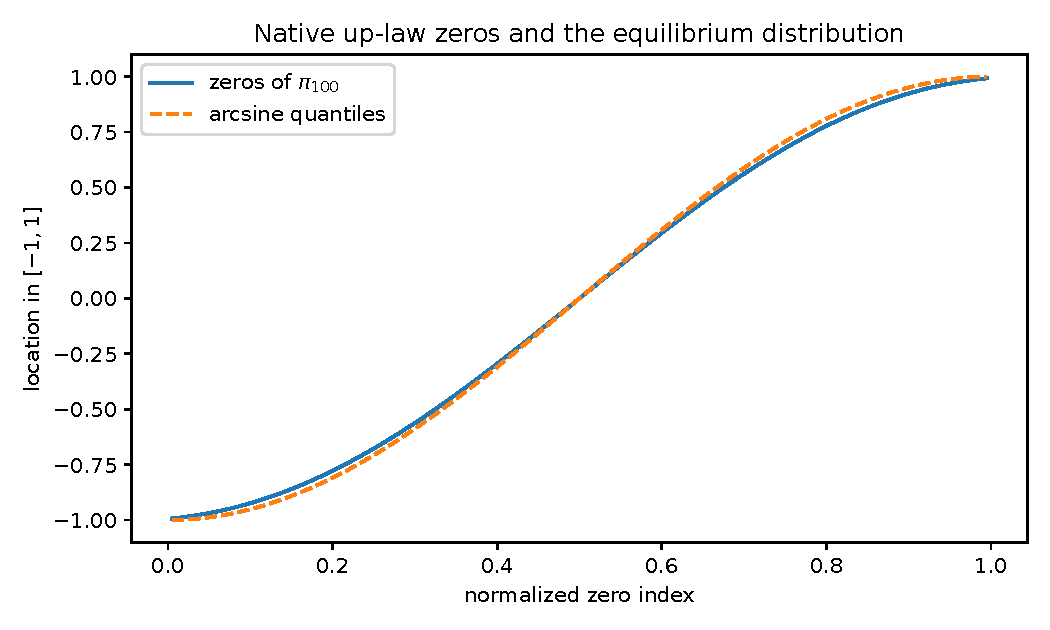
\includegraphics[width=0.82\textwidth]{zero_quantiles.pdf}
\caption{Zeros of $\pi_{100}$, computed as eigenvalues of the finite Jacobi
matrix, against the arcsine quantiles.  This is a numerical illustration of
\cref{eq:arcsine-zero-limit}, not an additional proof.}
\label{fig:zero-quantiles}
\end{figure}

\subsection{Strong norm asymptotics and a Fabius--Szeg\H{o} constant}
The logarithmic endpoint condition permits the strong norm form of
Szeg\H{o}'s theorem.  Define
\begin{equation}
 \mathcal C_{\!F}
 =2\pi\exp\left[
   \frac1\pi\int_0^\pi
      \log\bigl(w(\cos\theta)\sin\theta\bigr)\dd\theta
 \right].
 \label{eq:fabius-szego-constant}
\end{equation}
The integral is finite by \cref{thm:up-szego}, and
$\mathcal C_{\!F}>0$.

\begin{theorem}[Strong monic norm asymptotic]
\label{thm:strong-norm}
The native monic norms satisfy
\begin{equation}
 \boxed{4^nH_n\longrightarrow\mathcal C_{\!F}.}
 \label{eq:strong-norm}
\end{equation}
Consequently,
\begin{equation}
 \mathcal C_{\!F}
   =\prod_{n=1}^{\infty}4\beta_n,
 \label{eq:szego-beta-product}
\end{equation}
where the product converges to a finite positive number.
\end{theorem}

\begin{proof}
Equation \cref{eq:strong-norm} is Szeg\H{o}'s strong norm theorem in monic
normalization; the constant is fixed by checking the model weight $w\equiv1$,
for which $4^nH_n\to\pi$.  Since $H_0=1$ and
$H_n=\prod_{j=1}^{n}\beta_j$, one has the exact finite identity
$4^nH_n=\prod_{j=1}^{n}4\beta_j$.  Passing to the limit proves
\cref{eq:szego-beta-product}.
\end{proof}

The partial product through $n=200$ is
\begin{equation}
 \prod_{n=1}^{200}4\beta_n
 =0.00213943931416523273491231\ldots.
 \label{eq:szego-partial-200}
\end{equation}
This number is \emph{not} presented as an accurate decimal evaluation of
$\mathcal C_{\!F}$: the convergence is slow enough that the uncomputed tail is
material.  Its role is to certify positivity and provide data for future
extrapolation.

\begin{corollary}[Hankel determinant asymptotic]
\label{cor:hankel-asymptotic}
As $N\to\infty$,
\begin{equation}
 \boxed{
 \Delta_N=\mathcal C_{\!F}^{\,N}
          2^{-N(N-1)}\exp\bigl(\smallo(N)\bigr).}
 \label{eq:hankel-asymptotic}
\end{equation}
In particular,
\begin{equation}
 \Delta_N^{1/N^2}\longrightarrow\frac12.
 \label{eq:hankel-capacity}
\end{equation}
\end{corollary}

\begin{proof}
The Gram identity gives $\Delta_N=\prod_{n=0}^{N-1}H_n$.  From
\cref{eq:strong-norm},
$\log H_n=\log\mathcal C_{\!F}-n\log4+\smallo(1)$.  Summation gives
\begin{align*}
 \log\Delta_N
 &=N\log\mathcal C_{\!F}
   -\log4\sum_{n=0}^{N-1}n+\smallo(N)\\
 &=N\log\mathcal C_{\!F}-N(N-1)\log2+\smallo(N),
\end{align*}
which is \cref{eq:hankel-asymptotic}.  Divide by $N^2$ and exponentiate to
obtain \cref{eq:hankel-capacity}.
\end{proof}

The capacity-scale limit $1/2$ is universal for regular measures on
$[-1,1]$; all Fabius-specific information surviving at the next exponential
scale is compressed into $\mathcal C_{\!F}$.

\section{Christoffel reconstruction from rational moments}
\label{sec:christoffel}

Christoffel functions turn the moment matrix into a local density estimator.
For $N\ge1$, let $\mathcal P_{N-1}$ be the polynomials of degree below $N$
and define
\begin{equation}
 \lambda_N(x)
 =\min\left\{
   \int_{-1}^{1}|P(t)|^2w(t)\dd t:
   P\in\mathcal P_{N-1},\ P(x)=1
 \right\}.
 \label{eq:christoffel-variational}
\end{equation}
If $p_n=\pi_n/\sqrt{H_n}$, the Christoffel--Darboux kernel and Christoffel
function are
\begin{equation}
 K_N(x,y)=\sum_{n=0}^{N-1}p_n(x)p_n(y),
 \qquad
 \lambda_N(x)=\frac1{K_N(x,x)}.
 \label{eq:christoffel-kernel}
\end{equation}

\subsection{Moment-matrix formula and exact arithmetic}
Put
\begin{equation}
 M_N=[m_{j+k}]_{j,k=0}^{N-1},
 \qquad
 v_N(x)=(1,x,\ldots,x^{N-1})^{\mathsf T}.
 \label{eq:moment-vector}
\end{equation}

\begin{proposition}[Inverse-Hankel formula]
\label{prop:inverse-hankel-christoffel}
For every real $x$,
\begin{equation}
 K_N(x,x)=v_N(x)^{\mathsf T}M_N^{-1}v_N(x),
 \qquad
 \boxed{\lambda_N(x)=
 \frac1{v_N(x)^{\mathsf T}M_N^{-1}v_N(x)}.}
 \label{eq:inverse-hankel-christoffel}
\end{equation}
In particular, $\lambda_N(x)\in\Q$ whenever $x\in\Q$.
\end{proposition}

\begin{proof}
For a coefficient vector $c$, the squared norm of
$P(t)=c^{\mathsf T}v_N(t)$ is $c^{\mathsf T}M_Nc$.  Minimize this positive
definite quadratic form subject to $c^{\mathsf T}v_N(x)=1$.  A Lagrange
multiplier gives
$c=M_N^{-1}v_N(x)/(v_N(x)^{\mathsf T}M_N^{-1}v_N(x))$, and substitution
yields \cref{eq:inverse-hankel-christoffel}.  The entries of $M_N$ and its
inverse are rational, so rational $x$ gives a rational value.
\end{proof}

The proposition makes every Christoffel value at a dyadic point an exact
rational expression in the Bell--Bernoulli moment data.  It does not sample
$w$ at that point; it infers local density from the first $2N-2$ moments.

\subsection{Bulk reconstruction theorem}
For positive continuous weights, the M\'at\'e--Nevai--Totik asymptotic is
\cite{MateNevaiTotik,TotikChristoffel,DankaTotik}
\begin{equation}
 N\lambda_N(x)\longrightarrow
 \pi w(x)\sqrt{1-x^2},
 \qquad -1<x<1.
 \label{eq:christoffel-bulk}
\end{equation}
The convergence is locally uniform wherever the weight is continuous and
positive.  Those hypotheses hold on every compact subinterval of $(-1,1)$.

\begin{theorem}[Pointwise reconstruction of Rvachev's bump]
\label{thm:christoffel-reconstruction}
For every $x\in(-1,1)$,
\begin{equation}
 \boxed{
 w(x)=\Up(x)=\lim_{N\to\infty}
 \frac{N\lambda_N(x)}{\pi\sqrt{1-x^2}}.}
 \label{eq:up-christoffel-reconstruction}
\end{equation}
The convergence is locally uniform in $x$.
\end{theorem}

This is a reconstruction of a nowhere-analytic $C^\infty$ function from
finite rational moment matrices.  At a rational $x$, every approximant is a
rational number divided only by the displayed factor
$\pi\sqrt{1-x^2}$.  At the symmetry point the algebraic factor disappears.

\begin{corollary}[A canonical rational limit for $\pi$]
\label{cor:christoffel-pi}
Since $w(0)=1$,
\begin{equation}
 \boxed{N\lambda_N(0)\longrightarrow\pi.}
 \label{eq:christoffel-pi}
\end{equation}
Every term $N\lambda_N(0)$ is rational.
\end{corollary}

The first paired values are
\begin{align}
 \lambda_1(0)=\lambda_2(0)&=1,\notag\\
 \lambda_3(0)=\lambda_4(0)&=\frac{32}{57},\notag\\
 \lambda_5(0)=\lambda_6(0)&=
   \frac{26727424}{67149435}.
 \label{eq:first-christoffel-values}
\end{align}
Consequently,
\begin{equation}
 2\lambda_2(0)=2,
 \qquad
 4\lambda_4(0)=\frac{128}{57}=2.245614\ldots,
 \qquad
 6\lambda_6(0)=
 \frac{53454848}{22383145}=2.388174\ldots.
 \label{eq:first-christoffel-pi-values}
\end{equation}
Parity explains the repetitions: $p_{2j+1}(0)=0$, hence adding an odd
polynomial to the kernel does not change its central value.

\subsection{A moment reconstruction of the Fabius function itself}
For $0<x<1$, the translation identity $F(x)=w(x-1)$ turns
\cref{eq:up-christoffel-reconstruction} into
\begin{equation}
 \boxed{
 F(x)=\lim_{N\to\infty}
 \frac{N\lambda_N(x-1)}{\pi\sqrt{x(2-x)}}.}
 \label{eq:fabius-christoffel-reconstruction}
\end{equation}
Thus the full bounded Fabius function can be recovered from its even moments,
without direct recursion on dyadic intervals.  Formula
\cref{eq:fabius-christoffel-reconstruction} also proposes a new approximation
scheme for the inverse: solve the finite algebraic equation
\begin{equation}
 \frac{N\lambda_N(x-1)}{\pi\sqrt{x(2-x)}}=y
 \label{eq:christoffel-inverse-approx}
\end{equation}
for $x\in(0,1)$.  The left side is an explicit rational function times one
square root.  Bulk convergence controls this procedure away from $x=0,1$;
the endpoint Lambert-$W$ regime requires a separate double-scaling analysis.

\begin{remark}[Why the endpoint is a genuine second problem]
The factor $\sqrt{1-x^2}$ in \cref{eq:christoffel-bulk} belongs to the
universal equilibrium density.  Near $x=1$, it competes with the much smaller
logarithmic-square density $w(x)$.  Classical bulk asymptotics are therefore
not uniform on scales where $1-x$ shrinks with $N$.  Matching the Christoffel
kernel to the repository's Lambert-$W$ endpoint saddle is one of the most
promising open directions in \cref{sec:future}.
\end{remark}

\section{An alternating rational Jacobi product for \texorpdfstring{$\pi$}{pi}}
\label{sec:pi-product}

The center $x=0$ is special for an even measure.  Here the strong Szeg\H{o}
interior asymptotic becomes an exact product statement about alternating
Jacobi coefficients.

\subsection{Strong center asymptotics}
The strong interior Szeg\H{o} formula for an even weight gives
\begin{equation}
 p_{2M}(0)^2\longrightarrow\frac{2}{\pi w(0)}.
 \label{eq:strong-center-general}
\end{equation}
For the up-law $w(0)=1$, so the limit is $2/\pi$.

\begin{lemma}[Exact central product]
\label{lem:central-product}
For every $M\ge1$,
\begin{equation}
 \pi_{2M}(0)=(-1)^M\prod_{j=1}^{M}\beta_{2j-1},
 \label{eq:monic-center-product}
\end{equation}
and
\begin{equation}
 p_{2M}(0)^2
 =\prod_{j=1}^{M}\frac{\beta_{2j-1}}{\beta_{2j}}.
 \label{eq:orthonormal-center-product}
\end{equation}
\end{lemma}

\begin{proof}
Set $x=0$ in \cref{eq:monic-recurrence}.  Odd polynomials vanish and
$\pi_{2M}(0)=-\beta_{2M-1}\pi_{2M-2}(0)$, which iterates to
\cref{eq:monic-center-product}.  Also
$H_{2M}=\prod_{n=1}^{2M}\beta_n$.  Divide the square of
\cref{eq:monic-center-product} by $H_{2M}$ to obtain
\cref{eq:orthonormal-center-product}.
\end{proof}

\begin{theorem}[Fabius--Jacobi product for $\pi$]
\label{thm:pi-product}
The rational partial products
\begin{equation}
 \Pi_M=2\prod_{j=1}^{M}\frac{\beta_{2j}}{\beta_{2j-1}}
 \label{eq:pi-partial-product}
\end{equation}
converge to $\pi$.  Equivalently,
\begin{equation}
 \boxed{
 \pi=2\prod_{j=1}^{\infty}
          \frac{\beta_{2j}}{\beta_{2j-1}}.}
 \label{eq:pi-infinite-product}
\end{equation}
\end{theorem}

\begin{proof}
By \cref{lem:central-product},
$\Pi_M=2/p_{2M}(0)^2$.  Apply \cref{eq:strong-center-general} with
$w(0)=1$.
\end{proof}

The formula is not a generic tautology.  For a general even Szeg\H{o} weight,
identical reasoning gives
\begin{equation}
 \boxed{
 \pi w(0)=2\prod_{j=1}^{\infty}
          \frac{\beta_{2j}}{\beta_{2j-1}}.}
 \label{eq:general-center-product}
\end{equation}
The up-law is distinguished by the exact normalization $w(0)=1$, so the
spectral product isolates $\pi$ itself.

\subsection{Hankel-determinant form}
Substitution of
$\beta_n=\Delta_{n+1}\Delta_{n-1}/\Delta_n^2$ into
\cref{eq:pi-infinite-product} gives a formula involving only exact moment
Hankel determinants:
\begin{equation}
 \boxed{
 \pi=2\prod_{j=1}^{\infty}
 \frac{\Delta_{2j+1}\Delta_{2j-1}^{\,3}}
      {\Delta_{2j}^{\,3}\Delta_{2j-2}}.}
 \label{eq:pi-hankel-product}
\end{equation}
Every determinant in \cref{eq:pi-hankel-product} is a rational expression in
the Fabius moments, which in turn are generated by Bernoulli/Bell data or the
triangular recurrence.  This supplies a direct arithmetic chain
\begin{equation}
 \text{Bernoulli cumulants}
 \longrightarrow \text{Bell moments}
 \longrightarrow \text{Hankel determinants}
 \longrightarrow \pi.
 \label{eq:bernoulli-to-pi-chain}
\end{equation}

\subsection{Exact harmonic mean of the product approximants}
Set $\Pi_0=2$.  Since $p_{2m+1}(0)=0$,
\begin{equation}
 K_{2M}(0,0)=\sum_{m=0}^{M-1}p_{2m}(0)^2
 =2\sum_{m=0}^{M-1}\frac1{\Pi_m}.
 \label{eq:center-kernel-products}
\end{equation}

\begin{theorem}[Christoffel--product harmonic mean]
\label{thm:harmonic-mean}
For every $M\ge1$,
\begin{equation}
 \boxed{
 2M\lambda_{2M}(0)
 =\frac{M}{\displaystyle\sum_{m=0}^{M-1}\Pi_m^{-1}}.}
 \label{eq:harmonic-mean}
\end{equation}
Thus the Christoffel approximant is exactly the harmonic mean of
$\Pi_0,\ldots,\Pi_{M-1}$.
\end{theorem}

\begin{proof}
Invert \cref{eq:center-kernel-products} and multiply by $2M$.
\end{proof}

This identity explains why the direct products converge much faster in the
experiments than $2M\lambda_{2M}(0)$: the latter averages the entire history,
including the crude early values.

\begin{corollary}[Conditional first correction]
\label{cor:christoffel-first-correction}
Suppose
\begin{equation}
 \mathcal S_F=
 \sum_{m=0}^{\infty}\left(\frac1{\Pi_m}-\frac1\pi\right)
 \label{eq:christoffel-shift-constant}
\end{equation}
converges.  Then
\begin{equation}
 2M\lambda_{2M}(0)
 =\pi-\frac{\pi^2\mathcal S_F}{M}+\smallo(M^{-1}).
 \label{eq:christoffel-first-correction}
\end{equation}
\end{corollary}

\begin{proof}
The denominator in \cref{eq:harmonic-mean} is
$M/\pi+\mathcal S_F+\smallo(1)$.  Expand its reciprocal.
\end{proof}

The convergence assumed here follows, for example, from the product-error
conjecture in \cref{conj:beta-rate}.  The data suggest
$M(\pi-2M\lambda_{2M}(0))$ approaches a finite positive constant; at $M=100$
it is approximately $5.8867251451$.

\subsection{Initial rational products}
The first two exact products and several high-precision values are
\begin{align}
 \Pi_1&=\frac{64}{25}=2.56,\notag\\
 \Pi_2&=\frac{53454848}{19541211}=2.7354931073616676\ldots,\notag\\
 \Pi_3&=2.8320987418684373\ldots,\qquad
 \Pi_4=2.9033763206778567\ldots,\notag\\
 \Pi_5&=2.9457847614454995\ldots,\qquad
 \Pi_{10}=3.0478239630996334\ldots,\notag\\
 \Pi_{20}&=3.1010805882480384\ldots,\qquad
 \Pi_{50}=3.1298973222596123\ldots,\notag\\
 \Pi_{100}&=3.1373662375494674\ldots.
 \label{eq:pi-product-values}
\end{align}
The fact that these values increase and remain below $\pi$ is empirical at
present; convergence itself is proved by \cref{thm:pi-product}.

\begin{figure}[htbp]
\centering
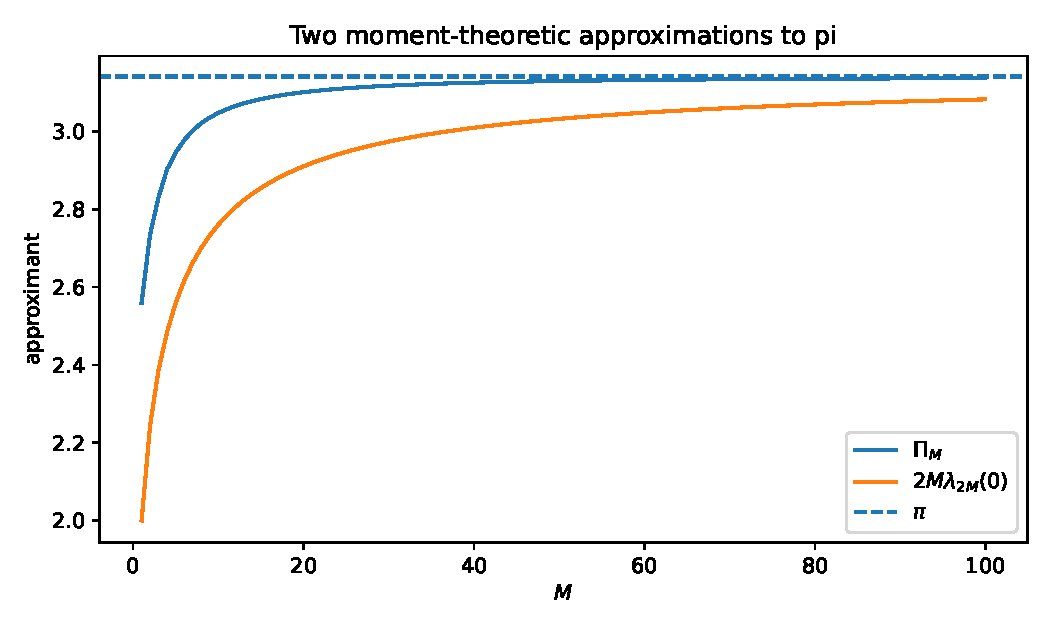
\includegraphics[width=0.82\textwidth]{pi_approximants.pdf}
\caption{The direct rational products $\Pi_M$ and the exact Christoffel
harmonic means $2M\lambda_{2M}(0)$.  Both converge to $\pi$; monotone approach
from below is conjectural.}
\label{fig:pi-approximants}
\end{figure}

\section{Gauss quadrature and Pad\'e approximation of the Cauchy transform}
\label{sec:gauss-pade}

The repository already proves the Laurent expansion and the affine-difference
renormalization of the up-law Cauchy transform.  Native orthogonal polynomials
supply the missing continued-fraction and optimal-quadrature layer.

\subsection{Exact Gaussian rules}
Let $x_{N,1}<\cdots<x_{N,N}$ be the zeros of $\pi_N$.  They are simple and
belong to $(-1,1)$.  Define
\begin{equation}
 \omega_{N,j}=\lambda_N(x_{N,j})
 =\frac1{K_N(x_{N,j},x_{N,j})}>0.
 \label{eq:gauss-weights}
\end{equation}

\begin{theorem}[Native up-law Gauss quadrature]
\label{thm:gauss-quadrature}
For every polynomial $P$ of degree at most $2N-1$,
\begin{equation}
 \boxed{
 \int_{-1}^{1}P(x)w(x)\dd x
 =\sum_{j=1}^{N}\omega_{N,j}P(x_{N,j}).}
 \label{eq:gauss-quadrature}
\end{equation}
The nodes are algebraic, the weights are positive algebraic numbers, and all
symmetric sums required to verify \cref{eq:gauss-quadrature} belong to $\Q$.
\end{theorem}

The first rules are especially simple:
\begin{align}
 N=1:&\qquad x_{1,1}=0,
  & \omega_{1,1}&=1;\notag\\
 N=2:&\qquad x_{2,1},x_{2,2}=\mp\frac13,
  & \omega_{2,1}=\omega_{2,2}&=\frac12;\label{eq:gauss-two}\\
 N=3:&\qquad x_{3,1},x_{3,2},x_{3,3}
   =-\sqrt{\frac{19}{75}},0,\sqrt{\frac{19}{75}},
  & \omega_{3,2}&=\frac{32}{57},\quad
    \omega_{3,1}=\omega_{3,3}=\frac{25}{114}.
 \label{eq:gauss-three}
\end{align}
Thus the two-node rule integrates exactly through degree three and the
three-node rule through degree five against the non-elementary density $w$.
These formulae are useful for integrals involving $F$ because
$F(x)=w(x-1)$ on $[0,1]$.

\subsection{The Jacobi continued fraction}
For $z\in\C\setminus[-1,1]$, define
\begin{equation}
 \mathcal R(z)=\int_{-1}^{1}\frac{w(x)}{z-x}\dd x.
 \label{eq:cauchy-transform}
\end{equation}
At infinity,
\begin{equation}
 \mathcal R(z)=\sum_{k=0}^{\infty}\frac{m_k}{z^{k+1}},
 \qquad |z|>1,
 \label{eq:cauchy-moment-series}
\end{equation}
with the exact finite remainders already formalized in the repository.
Stieltjes--Markov theory~\cite{Chihara,BakerGravesMorris} gives the $J$-fraction
\begin{equation}
 \boxed{
 \mathcal R(z)=
 \cfrac1{z-\cfrac{\beta_1}{z-
        \cfrac{\beta_2}{z-
        \cfrac{\beta_3}{\ddots}}}}.}
 \label{eq:j-fraction}
\end{equation}
The fraction converges locally uniformly off $[-1,1]$.

Let
\begin{equation}
 Q_{N-1}(z)=\int_{-1}^{1}
 \frac{\pi_N(z)-\pi_N(x)}{z-x}w(x)\dd x.
 \label{eq:second-kind-polynomial}
\end{equation}
Then $Q_{N-1}\in\Q[z]$ has degree $N-1$ and the $N$th convergent of
\cref{eq:j-fraction} is $Q_{N-1}/\pi_N$.

\begin{theorem}[Gauss--Pad\'e identity and exact error]
\label{thm:pade-error}
The rational function $Q_{N-1}/\pi_N$ is the $[N-1/N]$ Pad\'e approximant of
\cref{eq:cauchy-moment-series} at infinity.  Moreover,
\begin{equation}
 \boxed{
 \mathcal R(z)-\frac{Q_{N-1}(z)}{\pi_N(z)}
 =\frac1{\pi_N(z)^2}
   \int_{-1}^{1}\frac{\pi_N(x)^2}{z-x}w(x)\dd x.}
 \label{eq:pade-exact-error}
\end{equation}
For real $z>1$ this error is strictly positive and satisfies
\begin{equation}
 \frac{H_N}{(z+1)\pi_N(z)^2}
 \le
 \mathcal R(z)-\frac{Q_{N-1}(z)}{\pi_N(z)}
 \le
 \frac{H_N}{(z-1)\pi_N(z)^2}.
 \label{eq:pade-two-sided-error}
\end{equation}
\end{theorem}

\begin{proof}
From \cref{eq:second-kind-polynomial},
\begin{equation*}
 \pi_N(z)\mathcal R(z)-Q_{N-1}(z)
 =\int\frac{\pi_N(x)}{z-x}\dd\mu(x).
\end{equation*}
The polynomial
$(\pi_N(z)-\pi_N(x))/(z-x)$ has degree $N-1$ in $x$, so it is orthogonal to
$\pi_N(x)$.  Therefore
\begin{equation*}
 \pi_N(z)\int\frac{\pi_N(x)}{z-x}\dd\mu(x)
 =\int\frac{\pi_N(x)^2}{z-x}\dd\mu(x),
\end{equation*}
which proves \cref{eq:pade-exact-error}.  Expansion at infinity and
orthogonality show that the first $2N$ Laurent coefficients agree, giving the
Pad\'e order.  For $z>1$,
$(z+1)^{-1}\le(z-x)^{-1}\le(z-1)^{-1}$ on the support; integration gives
\cref{eq:pade-two-sided-error}.
\end{proof}

Partial fractions recover the Gaussian rule:
\begin{equation}
 \frac{Q_{N-1}(z)}{\pi_N(z)}
 =\sum_{j=1}^{N}\frac{\omega_{N,j}}{z-x_{N,j}}.
 \label{eq:pade-gauss-partial-fractions}
\end{equation}
Thus Gaussian quadrature and Pad\'e approximation are two faces of the same
finite Jacobi truncation.

The first nontrivial convergents are
\begin{align}
 \mathcal R_1(z)&=\frac1z,\notag\\
 \mathcal R_2(z)&=\frac{z}{z^2-1/9},\notag\\
 \mathcal R_3(z)&=\frac{z^2-32/225}{z(z^2-19/75)}.
 \label{eq:first-pade-convergents}
\end{align}
For rational $z>1$, each value is rational and is a certified lower bound for
$\mathcal R(z)$; \cref{eq:pade-two-sided-error} provides a fully explicit
rational error interval.

\subsection{Coupling to dyadic renormalization}
The repository proves
\begin{equation}
 \mathcal R'(z)=2\bigl(\mathcal R(2z+1)-\mathcal R(2z-1)\bigr),
 \qquad z\in\C\setminus[-1,1].
 \label{eq:cauchy-renormalization}
\end{equation}
Equations \cref{eq:j-fraction,eq:cauchy-renormalization} are complementary:
the first is spectral and nonlinear in the sequence $\beta_n$, while the
second is dyadic and linear in the function $\mathcal R$.  Substitution of the
finite convergents $\mathcal R_N$ into \cref{eq:cauchy-renormalization} creates
explicit rational residuals
\begin{equation}
 \mathfrak E_N(z)=
 \mathcal R_N'(z)-2\bigl(\mathcal R_N(2z+1)-\mathcal R_N(2z-1)\bigr).
 \label{eq:pade-renormalization-residual}
\end{equation}
The exact error formula bounds $\mathfrak E_N$ on compact subsets of the slit
plane.  Studying its poles and signs may convert the dyadic functional law
into new inequalities for the Jacobi coefficients; this program is stated
more precisely in \cref{sec:future}.

\section{The Legendre--Gaunt determinant bridge}
\label{sec:legendre-gaunt}

The preceding sections used only the native moments.  We now connect them to
the repository's exact Fourier--Legendre expansion, thereby closing a finite
algebraic circuit between the classical and native orthogonal systems.

\subsection{Exact Legendre data}
Let $P_n$ be the standard Legendre polynomial, $P_n(1)=1$.  The repository
proves an absolutely and uniformly convergent expansion
\begin{equation}
 w(x)=\sum_{r=0}^{\infty}c_rP_{2r}(x),
 \qquad
 c_r=\frac{4r+1}{2}\int_{-1}^{1}w(x)P_{2r}(x)\dd x,
 \label{eq:up-legendre-series}
\end{equation}
with $c_r\in\Q$.  Only even degrees occur because $w$ is even.

For $N\ge1$, form the Gram matrix of the first $N$ Legendre polynomials in the
\emph{up} inner product:
\begin{equation}
 G_N=\left[
  \int_{-1}^{1}P_j(x)P_k(x)w(x)\dd x
 \right]_{j,k=0}^{N-1}.
 \label{eq:legendre-gram}
\end{equation}
For $N=0$, set $G_0$ to be the empty $0\mathbin{\times}0$ Gram matrix.  This
standard convention extends the preceding $N\ge1$ definition and gives
$\det G_0=1$.

\subsection{Finite Gaunt expansion}
The Gaunt integral is
\begin{equation}
 \int_{-1}^{1}P_j(x)P_k(x)P_\ell(x)\dd x
 =2\begin{pmatrix}j&k&\ell\\0&0&0\end{pmatrix}^{\!2}.
 \label{eq:gaunt-integral}
\end{equation}
It vanishes unless the triangle inequalities hold and $j+k+\ell$ is even.
Consequently the apparently infinite substitution of
\cref{eq:up-legendre-series} into \cref{eq:legendre-gram} truncates exactly.

\begin{theorem}[Finite rational Gaunt matrix]
\label{thm:finite-gaunt-matrix}
For $0\le j,k<N$,
\begin{equation}
 \boxed{
 (G_N)_{jk}=
 2\sum_{r\ge0}c_r
 \begin{pmatrix}j&k&2r\\0&0&0\end{pmatrix}^{\!2},}
 \label{eq:finite-gaunt-matrix}
\end{equation}
where only
$|j-k|\le2r\le j+k$ contribute.  Thus every entry of $G_N$ is a finite
rational sum.
\end{theorem}

For completeness, if $j+k+\ell=2s$, the squared symbol is
\begin{equation}
 \begin{pmatrix}j&k&\ell\\0&0&0\end{pmatrix}^{\!2}
 =\frac{s!^2}{(s-j)!^2(s-k)!^2(s-\ell)!^2}
  \frac{(2s-2j)!(2s-2k)!(2s-2\ell)!}{(2s+1)!};
 \label{eq:wigner-factorial}
\end{equation}
otherwise it is zero.  Formula \cref{eq:wigner-factorial} makes the
rationality in \cref{eq:finite-gaunt-matrix} completely explicit.

\subsection{Determinants recover the native recurrence}
The leading coefficient of $P_n$ is
\begin{equation}
 L_n=2^{-n}\binom{2n}{n}.
 \label{eq:legendre-leading}
\end{equation}
Let $D_N=\det G_N$, so in particular the empty-determinant convention gives
$D_0=1$.  The triangular change of basis from monomials to
$P_0,\ldots,P_{N-1}$ has determinant $\prod_{j=0}^{N-1}L_j$.  Hence:

\begin{theorem}[Legendre--Hankel determinant identity]
\label{thm:legendre-hankel}
For every $N\ge0$,
\begin{equation}
 \boxed{
 D_N=\left(\prod_{j=0}^{N-1}L_j^2\right)\Delta_N.}
 \label{eq:legendre-hankel}
\end{equation}
Consequently, for $n\ge1$,
\begin{equation}
 \boxed{
 \beta_n=
 \left(\frac{n}{2n-1}\right)^2
 \frac{D_{n+1}D_{n-1}}{D_n^2}.}
 \label{eq:beta-gaunt-determinants}
\end{equation}
\end{theorem}

\begin{proof}
Writing the Legendre coefficient vector as a triangular matrix times the
monomial coefficient vector gives $G_N=A_NM_NA_N^{\mathsf T}$, with
$\det A_N=\prod_{j<N}L_j$.  This proves
\cref{eq:legendre-hankel}.  Substitute it into
$\beta_n=\Delta_{n+1}\Delta_{n-1}/\Delta_n^2$.  The products telescope to
$(L_{n-1}/L_n)^2$, and
$L_n/L_{n-1}=(2n-1)/n$.
\end{proof}

\begin{remark}[Exact Lean crosswalk and indexing]
Equation \eqref{eq:legendre-hankel} is the specialization
\path{upLegendreGramDet_eq_prod_leadingCoeff_sq_mul_hankelDet}.  The theorem
\path{gramStieltjesJacobiSubdiagonal_upMoment_eq_upLegendreGramDet_ratio} and its
rational-cast companion
\path{rvachevJacobiSubdiagonalRat_cast_eq_upLegendreGramDet_ratio} use index $k\ge0$
for the conventional coefficient $\beta_{k+1}$; replacing $k$ by $n-1$ gives
exactly \eqref{eq:beta-gaunt-determinants}.  Their proof is the displayed
$G=C^{\mathsf T}HC$ determinant argument and does not depend on the separately
formalized finite Gaunt entry expansion.  The latter is supplied by
\path{LegendreGaunt.lean} and \path{FabiusLegendreGaunt.lean}; only its
Wigner/\(3j\) identification and factorial closed form remain outside Lean.
The determinant identity, $D_0=1$, the
leading-coefficient quotient, and the real Gram cross-ratio hold for every
\path{BoundedFabius}; entry-as-integral, strict positivity, and the rational-cast
bridge require \path{IsFabius}.  Without Hankel nonvanishing, the generic and real
Gram cross-ratios are unconditional only through totalized division: a zero middle
determinant makes both sides zero and does not supply a nonsingular Jacobi recurrence.
The executable rational continuation catalogued in
\cref{sec:native-op} computes the same finite Legendre entries directly from
rational coefficients and moments, casts its matrix and determinant to these
real objects, and proves the corresponding rational norm and zero-based Jacobi
determinant ratios.  The newer Gaunt modules prove that this entry is also the
finite rational Gaunt sum and cast that formula to the real up-law Gram matrix.
Neither route uses the Wigner identity or \cref{eq:wigner-factorial}.
\end{remark}

A low-degree check is instructive.  From the moments,
\begin{equation}
 G_3=
 \begin{pmatrix}
 1&0&-1/3\\
 0&1/9&0\\
 -1/3&0&11/75
 \end{pmatrix},
 \qquad
 D_3=\frac8{2025}.
 \label{eq:first-gaunt-matrix}
\end{equation}
Since $D_1=1$ and $D_2=1/9$, \cref{eq:beta-gaunt-determinants} gives
\begin{equation}
 \beta_2=\left(\frac23\right)^2
 \frac{(8/2025)\cdot1}{(1/9)^2}=\frac{32}{225},
 \label{eq:gaunt-beta-check}
\end{equation}
matching \cref{eq:low-jacobi-data}.

\subsection{Christoffel functions directly in the Legendre basis}
Let
\begin{equation}
 \mathbf P_N(x)=(P_0(x),\ldots,P_{N-1}(x))^{\mathsf T}.
 \label{eq:legendre-vector}
\end{equation}
Basis invariance of the reproducing kernel gives
\begin{equation}
 \boxed{
 K_N(x,x)=\mathbf P_N(x)^{\mathsf T}G_N^{-1}\mathbf P_N(x).}
 \label{eq:christoffel-legendre-basis}
\end{equation}
Combining \cref{eq:finite-gaunt-matrix,eq:christoffel-legendre-basis} with
\cref{eq:up-christoffel-reconstruction} yields a representation of $w(x)$
using only finite rational combinations of the existing exact Legendre
coefficients $c_r$.

This closes the promised circuit:
\begin{equation}
 \begin{gathered}
 \text{exact dyadic values of }F
 \longrightarrow c_r
 \longrightarrow G_N\text{ by Gaunt sums}
 \longrightarrow D_N
 \longrightarrow \beta_n\\
 \longrightarrow
 \begin{cases}
 \Pi_M\to\pi,\\
 \lambda_N(x)\to\pi w(x)\sqrt{1-x^2}/N,
 \end{cases}
 \longrightarrow w=\Up\longrightarrow F.
 \end{gathered}
 \label{eq:closed-spectral-circuit}
\end{equation}
Unlike the shifted-up self-reconstruction in the recent Legendre reports,
all intermediate matrices in \cref{eq:closed-spectral-circuit} are finite,
positive definite, and basis invariant.

\section{Numerical experiment and exact verification}
\label{sec:numerics}

The archive contains the standalone program
\path{fabius_frontier_experiments.py}.  It uses no sampled values of $F$ or
$w$.  Its only analytic input is the exact moment recurrence
\cref{eq:moment-recurrence}; all later quantities are generated by the native
three-term recurrence.

\subsection{Two arithmetic modes}
The program performs two independent calculations.
\begin{enumerate}
\item \textbf{Exact mode.}  Python's \texttt{Fraction} type generates the
      moments, polynomials, norms, $\beta_n$, $\Pi_M$, and central
      Christoffel approximants through degree $24$.  Exact assertions check
      \cref{eq:low-jacobi-data} through $\pi_4$ and $\beta_3$.
\item \textbf{High-precision mode.}  The same recurrence is evaluated with
      \texttt{mpmath} at $4{,}800$ decimal digits through $\beta_{200}$.
      Every coefficient through degree $24$ is compared with the independent
      exact calculation.  Positivity of every computed squared norm is also
      checked before any table or figure is written.
\end{enumerate}
The identity
\begin{equation}
 H_n=\int x^n\pi_n(x)w(x)\dd x
 \label{eq:numerical-norm-identity}
\end{equation}
reduces the recurrence to $\bigO(N^2)$ coefficient operations.  Thousands of
digits are nevertheless necessary because monomial coefficients and moments
cancel severely at high degree.  A failed longer trial was discarded in full;
none of its partial files or values are used in this report.

\subsection{Observed recurrence coefficients}
The validated values include:
\begin{table}[htbp]
\centering
\caption{Selected high-precision Jacobi coefficients.  The last column tests
the scaling proposed in \cref{conj:beta-rate}.}
\label{tab:beta-data}
\begin{tabular}{@{}rcc@{}}
\toprule
$n$ & $\beta_n$ &
$\displaystyle\frac{n^2(1/4-\beta_n)}{(\log_2n)^2}$\\
\midrule
10  & 0.218406233337115543 & 0.286299738281\\
20  & 0.234873012373991668 & 0.323934622747\\
40  & 0.243489365492140411 & 0.367794553321\\
60  & 0.246188400107704611 & 0.393271027136\\
80  & 0.247434883352791960 & 0.410759852630\\
100 & 0.248128725130487816 & 0.423932916190\\
150 & 0.248962552551866080 & 0.446697951249\\
200 & 0.249325249690015095 & 0.461932021189\\
\bottomrule
\end{tabular}
\end{table}
All $200$ computed coefficients satisfy
\begin{equation}
 0<\beta_1<\beta_2<\cdots<\beta_{200}<\frac14.
 \label{eq:computed-monotonicity}
\end{equation}
Only the endpoint limit $\beta_n\to1/4$ is proved; the strict inequalities in
\cref{eq:computed-monotonicity} are evidence for
\cref{conj:beta-monotone}.

\begin{figure}[htbp]
\centering

\includegraphics[width=0.82\textwidth]{jacobi_coefficients.pdf}
\caption{The computed native recurrence coefficients and the proved limit
$1/4$.}
\label{fig:jacobi-coefficients}
\end{figure}

\begin{figure}[htbp]
\centering
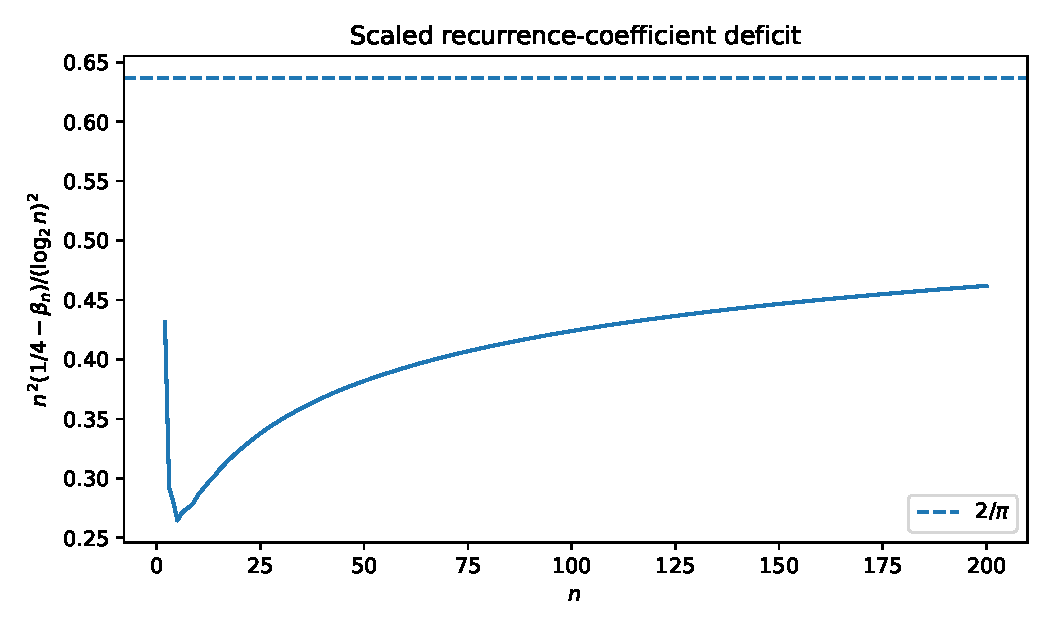
\includegraphics[width=0.82\textwidth]{scaled_jacobi_deficit.pdf}
\caption{The scaled deficit
$n^2(1/4-\beta_n)/(\log_2n)^2$.  The horizontal line is the conjectural limit
$2/\pi$, not a fitted value.}
\label{fig:scaled-beta-deficit}
\end{figure}

\subsection{Observed product errors}
For
$\Pi_M=2\prod_{j\le M}\beta_{2j}/\beta_{2j-1}$, the diagnostic
\begin{equation}
 E_M=\frac{M^2(\pi-\Pi_M)}{(\log_2M)^2}
 \label{eq:scaled-product-error}
\end{equation}
has the following values:
\begin{equation}
 \begin{array}{c|cccccc}
 M&10&20&50&75&100\\ \hline
 E_M&0.849723&0.867540&0.917911&0.941369&0.957485
 \end{array}
 \label{eq:product-error-data}
\end{equation}
The drift toward $1$ is substantially clearer than the corresponding drift
toward $2/\pi$ in \cref{tab:beta-data}; the alternating product cancels part
of the slowly varying lower-order structure.

\begin{figure}[htbp]
\centering
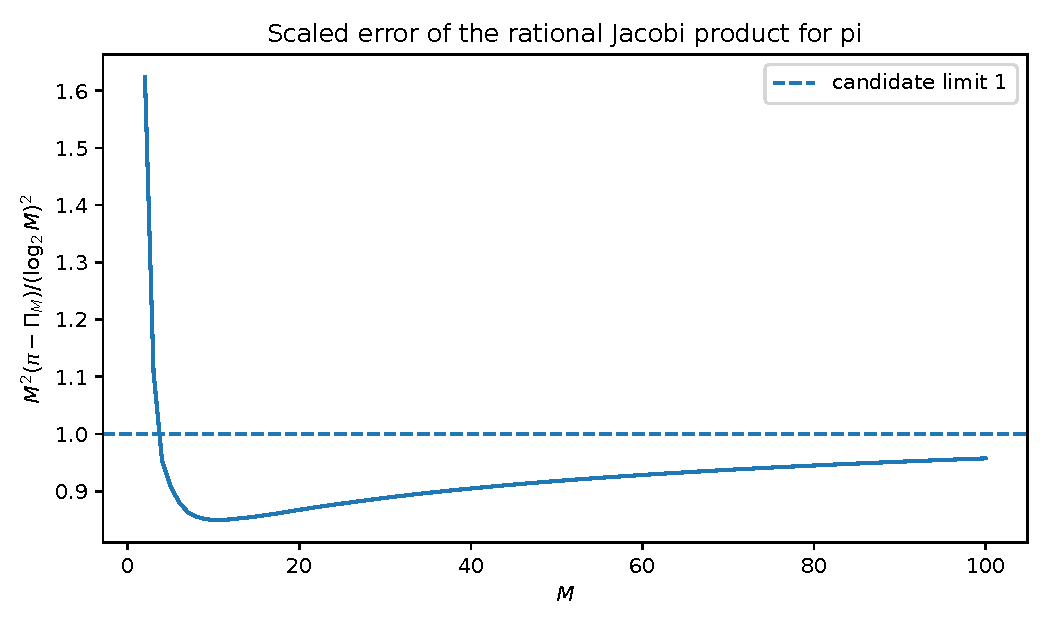
\includegraphics[width=0.82\textwidth]{pi_product_error.pdf}
\caption{Scaled error of the rational product.  The candidate limit $1$ is
part of \cref{conj:beta-rate}.}
\label{fig:pi-product-error}
\end{figure}

\subsection{Reproducibility and data products}
The command used for the archived run is
\begin{lstlisting}[style=pythonstyle]
python fabius_frontier_experiments.py \
    --degree 200 --dps 4800 --output .
\end{lstlisting}
It writes:
\begin{itemize}
\item \path{data/exact_low_degree.csv}, containing exact fractions;
\item \path{data/jacobi_coefficients.csv}, containing $\beta_1,\ldots,\beta_{200}$
      and scaled deficits;
\item \path{data/pi_product_approximants.csv}, containing the products,
      Christoffel harmonic means, and errors;
\item the five PDF figures reproduced in this report; and
\item \path{experiment_run.log}, the compact diagnostic transcript.
\end{itemize}
The script deliberately exposes its precision and degree as command-line
parameters.  Increasing the degree without increasing precision can silently
destroy positivity, so the program emits a warning below a conservative
precision threshold and checks exact low-degree overlap on every run.

\section{Conjectures suggested by the spectral data}
\label{sec:conjectures}

All statements in this section are open within the present report.  They are
ordered from structurally plausible to increasingly speculative.

\subsection{Monotonicity and one-sided rational approximants}

\begin{conjecture}[Strict Nevai approach]
\label{conj:beta-monotone}
For every $n\ge1$,
\begin{equation}
 0<\beta_n<\beta_{n+1}<\frac14.
 \label{eq:beta-monotone-conjecture}
\end{equation}
\end{conjecture}

If true, each ratio $\beta_{2j}/\beta_{2j-1}$ exceeds one.  Together with
\cref{thm:pi-product}, this would prove
\begin{equation}
 2<\Pi_1<\Pi_2<\cdots<\pi,
 \label{eq:pi-lower-bounds-conjectural}
\end{equation}
turning \cref{eq:pi-partial-product} into a canonical sequence of exact
rational lower bounds for $\pi$.  The harmonic-mean identity would then imply
that $2M\lambda_{2M}(0)$ is also increasing and lies below $\Pi_{M-1}<\pi$.
A proof may require a new comparison theorem for recurrence coefficients under
successive uniform convolution; generic log-concavity alone does not imply
\cref{eq:beta-monotone-conjecture}.

\subsection{A logarithmic-square correction at the Nevai edge}

\begin{conjecture}[Matched Jacobi and product rates]
\label{conj:beta-rate}
As $n,M\to\infty$,
\begin{align}
 \frac14-\beta_n
 &\sim\frac{2}{\pi}\frac{(\log_2n)^2}{n^2},
 \label{eq:beta-rate-conjecture}\\
 \pi-\Pi_M
 &\sim\frac{(\log_2M)^2}{M^2}.
 \label{eq:product-rate-conjecture}
\end{align}
\end{conjecture}

The appearance of the same logarithmic square as in
\cref{eq:endpoint-log-square} is natural: recurrence coefficients at order
$n$ resolve endpoint structure on a scale of order $n^{-2}$.  The numerical
constant $2/\pi$ is less obvious.  It is supported both by
\cref{fig:scaled-beta-deficit} and by the internal consistency calculation
below.

\begin{proposition}[Conditional matching of the two constants]
\label{prop:rate-matching}
Suppose $d_n=1/4-\beta_n$ has a sufficiently smooth regularly varying
asymptotic
\begin{equation}
 d_n\sim A\frac{(\log_2n)^2}{n^2},
 \qquad
 d_{n-1}-d_n\sim
 2A\frac{(\log_2n)^2}{n^3}.
 \label{eq:regular-difference-assumption}
\end{equation}
Then
\begin{equation}
 \pi-\Pi_M\sim
 \frac{\pi A}{2}\frac{(\log_2M)^2}{M^2}.
 \label{eq:conditional-product-rate}
\end{equation}
Thus the candidate coefficient $1$ in
\cref{eq:product-rate-conjecture} forces $A=2/\pi$.
\end{proposition}

\begin{proof}
Since $d_n\to0$,
$\log\beta_n=-\log4-4d_n+\bigO(d_n^2)$.  Therefore
\begin{align*}
 \log\frac{\pi}{\Pi_M}
 &=\sum_{j>M}\bigl(\log\beta_{2j}-\log\beta_{2j-1}\bigr)\\
 &=4\sum_{j>M}(d_{2j-1}-d_{2j})
   +\smallo\left(\frac{(\log M)^2}{M^2}\right).
\end{align*}
Using \cref{eq:regular-difference-assumption} at $n=2j$ and
$\sum_{j>M}j^{-3}\sim(2M^2)^{-1}$ gives
\begin{equation*}
 \log\frac{\pi}{\Pi_M}
 \sim\frac{A}{2}\frac{(\log_2M)^2}{M^2}.
\end{equation*}
Because this tends to zero, exponentiation gives
\cref{eq:conditional-product-rate}.
\end{proof}

A proof of \cref{eq:beta-rate-conjecture} likely lies beyond classical strong
Szeg\H{o} theory.  The weight vanishes at both endpoints faster than every
power, with a logarithmic-square exponent and dyadic lower-order oscillation.
A Riemann--Hilbert or nonlinear steepest-descent analysis adapted to this
``log-Gaussian hard edge'' appears necessary.

\subsection{Dyadic periodic modulation}
The repository's Mellin and Lambert analyses repeatedly produce periodic
functions of $\log_2$ of the scale.  It is therefore reasonable to expect a
smaller spectral echo.

\begin{conjecture}[Spectral dyadic ripple]
\label{conj:dyadic-ripple}
There exist bounded one-periodic functions $A_1,A_0$ such that, with
$L=\log_2n$,
\begin{equation}
 n^2\left(\frac14-\beta_n\right)
 =\frac{2}{\pi}L^2+L A_1(\{L\})+A_0(\{L\})+\smallo(1).
 \label{eq:dyadic-ripple}
\end{equation}
At least one of $A_1,A_0$ is nonconstant.
\end{conjecture}

The present range is too short to distinguish a genuine periodic ripple from
a long transient.  Testing \cref{eq:dyadic-ripple} requires a better
conditioned recurrence algorithm, preferably based on modified moments in a
Chebyshev basis rather than monomials.

\subsection{Strict log-concavity and strict Tur\'an inequalities}

\begin{conjecture}[Strict interior shape]
\label{conj:strict-logconcavity}
The function $\log w$ is strictly concave on $(-1,1)$.  Equivalently,
$\log F$ is strictly concave on $(0,1)$.  In particular,
\begin{equation}
 F(2x)^2>2F(x)F(4x),
 \qquad 0<x<\frac14.
 \label{eq:strict-turan-conjecture}
\end{equation}
\end{conjecture}

The conjecture should follow from equality-case analysis for Pr\'ekopa's
theorem applied to at least two nonproportional uniform summands, followed by
a limit argument.  A direct differential approach would amount to proving
strict decrease of $F(2x)/F(x)$.

\subsection{The central Christoffel shift}

\begin{conjecture}[Finite Christoffel shift]
\label{conj:christoffel-shift}
The series $\mathcal S_F$ in \cref{eq:christoffel-shift-constant} converges and
is positive.  Consequently
\begin{equation}
 M\bigl(\pi-2M\lambda_{2M}(0)\bigr)
 \longrightarrow \pi^2\mathcal S_F\in(0,\infty).
 \label{eq:christoffel-shift-conjecture}
\end{equation}
\end{conjecture}

Conjecture \ref{conj:beta-rate} implies absolute convergence because
$\pi-\Pi_M=\bigO((\log M)^2/M^2)$.  The computed value at $M=100$ is
$5.8867251451\ldots$; it should not yet be treated as a reliable estimate of
the limit.

\section{A geometric \texorpdfstring{$q$}{q}-uniform extension}
\label{sec:q-family}

The preceding structure is not isolated at the binary point.  It extends to a
natural geometric family that connects the repository's $q$-calculus to
log-concavity and Jacobi products.

\subsection{Definition, transform, and cumulants}
Let $0<q<1$, let $V_0,V_1,\ldots$ be independent uniform random variables on
$[-1,1]$, and put
\begin{equation}
 Y_q=\sum_{j=0}^{\infty}(1-q)q^jV_j.
 \label{eq:q-uniform-series}
\end{equation}
The coefficients sum to one, so $Y_q\in[-1,1]$.  Denote its even density by
$w_q$.  At $q=1/2$, $Y_q$ is exactly the up-law random variable $Y$ and
$w_{1/2}=w$.

The moment generating function is
\begin{equation}
 M_q(z)=\prod_{j=0}^{\infty}
 \frac{\sinh((1-q)q^jz)}{(1-q)q^jz}.
 \label{eq:q-mgf}
\end{equation}
Its even cumulants are
\begin{equation}
 \boxed{
 \kappa_{2r}(q)=
 \frac{2^{2r-1}B_{2r}}{r}
 \frac{(1-q)^{2r}}{1-q^{2r}},
 \qquad r\ge1.}
 \label{eq:q-cumulants}
\end{equation}
Thus rational $q$ gives rational cumulants, moments, Hankel determinants, and
Jacobi coefficients.  Formula \cref{eq:q-cumulants} specializes at $q=1/2$
to \cref{eq:cumulants}.

\subsection{Log-concavity and the Szeg\H{o} class}

\begin{theorem}[$q$-uniform log-concavity]
\label{thm:q-logconcavity}
For every $0<q<1$, the law of $Y_q$ is log-concave and its continuous density
$w_q$ is log-concave on $(-1,1)$.
\end{theorem}

\begin{proof}
Every finite partial sum in \cref{eq:q-uniform-series} is a convolution of
uniform log-concave measures.  The partial sums converge almost surely and in
distribution to $Y_q$.  Closure under convolution and weak limits proves
log-concavity of the limiting measure.  Convolution with the first uniform
summand gives a continuous density; its continuous representative is
log-concave.
\end{proof}

A useful exact endpoint relation follows by conditioning on $V_0$.  If
$T_q(t)=\Pr(Y_q\ge1-t)$, then for sufficiently small $t>0$,
\begin{equation}
 w_q(1-t)=\frac{T_q(t/q)}{2(1-q)}.
 \label{eq:q-endpoint-density-tail}
\end{equation}
A finite-coordinate small-box estimate, choosing
$N\asymp\log(1/t)/|\log q|$, gives
\begin{equation}
 -\log w_q(1-t)=\bigO\bigl(\log^2(1/t)\bigr).
 \label{eq:q-endpoint-log-square-bound}
\end{equation}
Hence the proof of \cref{thm:up-szego} applies verbatim and $w_q$ belongs to
the Szeg\H{o} class.  The sharper expected leading term is
\begin{equation}
 -\log w_q(1-t)
 \sim\frac{\log^2(1/t)}{2|\log q|},
 \label{eq:q-endpoint-leading-conjecture}
\end{equation}
but the exact normalization and periodic correction should be derived from a
separate Mellin analysis; \cref{eq:q-endpoint-leading-conjecture} is recorded
as a research target rather than used below.

\subsection{A continuum of Jacobi products}
Let $\beta_n(q)$ be the monic recurrence coefficients for
$w_q(x)\dd x$.  Rakhmanov and strong Szeg\H{o} theory give
\begin{equation}
 \beta_n(q)\longrightarrow\frac14
 \label{eq:q-nevai}
\end{equation}
and, by \cref{eq:general-center-product},
\begin{equation}
 \boxed{
 \pi w_q(0)=2\prod_{j=1}^{\infty}
 \frac{\beta_{2j}(q)}{\beta_{2j-1}(q)}.}
 \label{eq:q-center-product}
\end{equation}
At $q=1/2$, $w_q(0)=1$ and this is the new Fabius product
\cref{eq:pi-infinite-product}.

At the degenerate endpoint $q=0$, only $V_0$ remains and
$w_0\equiv1/2$.  The recurrence coefficients become those of monic Legendre
polynomials,
\begin{equation}
 \beta_n(0)=\frac{n^2}{4n^2-1}.
 \label{eq:legendre-beta}
\end{equation}
Then \cref{eq:q-center-product} reduces to a Wallis-type product for
$\pi/2$.  Thus the family continuously deforms the classical Wallis/Legendre
product into the Fabius product while preserving exact rationality whenever
$q\in\Q$.

This interpolation suggests a two-parameter research program: determine the
$q$-dependence of $w_q(0)$ and of the first correction to
$\beta_n(q)\to1/4$, and study whether monotonicity in $n$ or $q$ survives.

\section{Research program and formalization roadmap}
\label{sec:future}

The new results suggest several projects with sharply separated proof
requirements.  The first group is finite and algebraic; the last group needs
new asymptotic analysis.

\subsection{Prove monotonicity by a convolution flow}
The measure $\mu$ is obtained by repeatedly convolving with successively
smaller uniform laws.  Let $\mu^{(N)}$ be the law of the first $N$ summands and
$\beta_n^{(N)}$ its Jacobi coefficients.  A productive route to
\cref{conj:beta-monotone} is:
\begin{enumerate}
\item derive the response of finite Hankel determinants under convolution with
      a centered uniform law;
\item identify total-positivity or variation-diminishing inequalities that
      compare $\beta_{n+1}^{(N)}$ and $\beta_n^{(N)}$;
\item pass to the weak limit using moment convergence.
\end{enumerate}
The heat flow drives Jacobi data through a Toda-type system.  Uniform
convolution is not a semigroup, but a discrete analogue may exist through the
cumulant update
\begin{equation}
 \kappa_{2r}\longmapsto\kappa_{2r}
 +\frac{2^{2r-1}B_{2r}}{r}a^{2r}.
 \label{eq:uniform-cumulant-flow}
\end{equation}
Because the cumulant increment has alternating Bernoulli signs, naive
coefficientwise positivity is unlikely; Hankel total positivity is the more
plausible invariant.

\subsection{Derive the log-square Jacobi correction}
The principal analytic problem is to prove
\cref{eq:beta-rate-conjecture}.  A possible sequence of reductions is:
\begin{enumerate}
\item sharpen the endpoint formula to
\begin{equation}
 \log w(1-t)=
 -\frac{\log^2(1/t)}{2\log2}
 +A\bigl(\{\log_2(1/t)\}\bigr)\log(1/t)
 +B\bigl(\{\log_2(1/t)\}\bigr)+o(1),
 \label{eq:desired-endpoint-normal-form}
\end{equation}
with explicit periodic $A,B$;
\item insert this weight into the Riemann--Hilbert problem for the native
      orthogonal polynomials;
\item build an endpoint parametrix for an exponential of a squared logarithm,
      rather than a Jacobi power $t^\alpha$;
\item match it to the outer Szeg\H{o} parametrix and read off the $1/n^2$
      correction to the recurrence coefficients.
\end{enumerate}
The relevant endpoint scale should be found by balancing
$n\sqrt t$ against $\log(1/t)$, which is precisely where Lambert-$W$ enters.
This makes the repository's inverse-function asymptotics structurally relevant
to the native spectral problem, not merely analogous to it.

\subsection{Christoffel--Lambert double scaling}
Formula \cref{eq:fabius-christoffel-reconstruction} is a bulk statement.  A
uniform endpoint approximation would study
\begin{equation}
 x=x_N\downarrow0,
 \qquad
 \frac{N\lambda_N(x_N-1)}{\pi\sqrt{x_N(2-x_N)}}
 \label{eq:christoffel-endpoint-scale}
\end{equation}
on scales where the right side is exponentially small.  Three regimes should
be separated:
\begin{enumerate}
\item $x_N$ fixed: ordinary bulk asymptotics;
\item $x_N\to0$ slowly: a matching region controlled by the Szeg\H{o}
      function;
\item the critical edge: a new kernel depending on a Lambert-$W$ scaled
      coordinate and possibly on the fractional part of $\log_2(1/x_N)$.
\end{enumerate}
A successful analysis would give moment-based approximants to $F^{-1}(y)$
with rigorous error bounds and would identify the analogue of the Bessel
kernel for a logarithmic-square hard edge.

\subsection{Exploit the Pad\'e renormalization residual}
The residual \cref{eq:pade-renormalization-residual} is an explicit rational
function.  Several concrete questions are accessible computationally:
\begin{enumerate}
\item Does $\mathfrak E_N(z)$ have a fixed sign on $z>1$ after a simple
      normalization?
\item Do its poles interlace with the affine images of the Gauss nodes?
\item Can the exact error formula turn \cref{eq:cauchy-renormalization} into
      two-sided recursive bounds for $\mathcal R(z)$?
\item Does matching the Laurent expansion of $\mathfrak E_N$ reproduce the
      moment recurrence in a triangular way, and can the first unmatched term
      be expressed solely through $\beta_1,\ldots,\beta_N$?
\end{enumerate}
Positive answers would yield a structure-preserving numerical solver: compute
the Jacobi truncation, enforce the dyadic residual, and obtain certified bounds
without discretizing $w$.

\subsection{Arithmetic of Hankel and Gaunt determinants}
The dyadic-value literature studies denominators of $F(2^{-n})$.  The native
spectral data create a second arithmetic sequence:
\begin{equation}
 \Delta_N,\qquad D_N,\qquad \beta_N,
 \qquad \Pi_N.
 \label{eq:new-arithmetic-sequences}
\end{equation}
Promising questions include:
\begin{enumerate}
\item determine exact $2$-adic valuations of $\Delta_N$ and $\beta_N$;
\item isolate odd denominator factors coming from $2^{2r}-1$ in the moment
      recurrence;
\item test whether cancellations in
      \cref{eq:pi-hankel-product} admit finite valuation bounds uniform in
      $N$;
\item express $D_N$ directly through the rational Legendre coefficients
      $c_0,\ldots,c_{N-1}$ and classify the primes introduced by the Gaunt
      factorials.
\end{enumerate}
Because $\Pi_N\to\pi$, any unexpectedly strong denominator control would have
Diophantine consequences.  No irrationality claim is made here; the immediate
goal is an exact valuation theory parallel to the existing dyadic one.

\subsection{The geometric \texorpdfstring{$q$}{q}-surface}
For rational $q$, the whole moment/Jacobi/Gauss construction is exact.  One
can therefore sample the two-dimensional array $\beta_n(q)$ without evaluating
$w_q$.  Specific targets are:
\begin{enumerate}
\item prove the sharp endpoint coefficient in
      \cref{eq:q-endpoint-leading-conjecture};
\item find the $q$-analogue of \cref{eq:beta-rate-conjecture};
\item determine whether $n\mapsto\beta_n(q)$ is increasing for a full interval
      of $q$ values;
\item study the limits $q\downarrow0$ (Wallis/Legendre) and $q\uparrow1$
      after variance rescaling, where a Gaussian regime should emerge;
\item connect the cumulants \cref{eq:q-cumulants} to the repository's
      $q$-Pochhammer and Gaussian-binomial filters.
\end{enumerate}
This family provides a controlled deformation in which classical and Fabius
phenomena can be compared rather than studied in isolation.

\subsection{Numerical improvements}
The monomial recurrence becomes costly beyond a few hundred degrees.  Three
improvements are recommended:
\begin{enumerate}
\item compute modified moments in the Chebyshev or Legendre basis and apply a
      modified Chebyshev algorithm for the Jacobi coefficients;
\item use interval or ball arithmetic to certify signs of
      $1/4-\beta_n$ and $\beta_{n+1}-\beta_n$;
\item combine arbitrary precision with asymptotic preconditioning
      $\beta_n=1/4-d_n$ to avoid subtractive loss in the tail.
\end{enumerate}
The finite Gaunt formula \cref{eq:finite-gaunt-matrix} is particularly
attractive because it replaces ill-conditioned monomial Hankel matrices by a
near-orthogonal reference basis.

\subsection{Lean formalization order}
The repository already contains rational moments, positive Hankel matrices,
low-degree native polynomials, and the Cauchy renormalization. It now also contains
the finite scalar-naturality API, the all-degree rational native Jacobi layer,
the generic/Legendre Gram determinant change-of-basis layers, and executable
rational Legendre coefficient, entry, matrix, and determinant layers
catalogued in \cref{sec:native-op}: exact \(\Q\)-valued determinants, polynomial
coefficients, norms, zero diagonal, positive subdiagonals, determinant cross-ratio,
orthogonality, centered recurrence, and real-cast bridges, with zero-based index
\(n\) corresponding to \(\beta_{n+1}\).  The polynomial change-of-basis and Legendre
specializations catalogued there now formalize
\cref{eq:legendre-hankel,eq:beta-gaunt-determinants}.  The subsequent modules
\path{LegendreGaunt.lean} and \path{FabiusLegendreGaunt.lean} formalize the
finite integral, product-linearization, rational Gaunt-sum, and up-law
Gram-entry layers; the Wigner/\(3j\) identification and factorial formula remain
outside Lean.  The remaining formalization sequence is:
\begin{enumerate}
\item \textbf{Finite algebra:} the determinant change-of-basis and
      \cref{eq:legendre-hankel,eq:beta-gaunt-determinants} are supplied by
      \path{PolynomialMomentGramDeterminant.lean} and
      \path{FabiusLegendreHankelDeterminant.lean}; their executable rational
      coefficient and Gram refinements are supplied by
      \path{LegendrePolynomialRational.lean} and
      \path{FabiusLegendreRationalGram.lean}, with the displayed low-order
      certificates evaluated in \path{FabiusLegendreRationalGramValues.lean}.
      Formalize the remaining
      \cref{eq:inverse-hankel-christoffel,eq:monic-center-product,%
eq:orthonormal-center-product,eq:harmonic-mean}.  These need only finite
      linear algebra and the existing positivity and rational-native APIs.  The
      finite Gaunt integral and rational matrix-entry realization are already
      supplied by \path{LegendreGaunt.lean} and
      \path{FabiusLegendreGaunt.lean}.  Formalize only the remaining Wigner
      identity in \cref{eq:gaunt-integral} and the factorial form
      \cref{eq:wigner-factorial} if an explicit \(3j\)-symbol realization is
      desired.
\item \textbf{Quadrature and rational approximation:} define second-kind
      polynomials, prove \cref{eq:pade-exact-error}, and derive the Gaussian
      weights and exactness theorem.
\item \textbf{Convexity:} add a reusable notion of log-concave measure,
      closure under convolution and weak convergence, then prove
      \cref{thm:up-logconcave,cor:fabius-turan,cor:action-curvature}.
\item \textbf{Classical asymptotic interfaces:} formalize or import abstract
      versions of Rakhmanov, strong Szeg\H{o}, and Christoffel asymptotics.
      The Fabius-specific work then reduces to support, positivity, continuity,
      and the endpoint integrability estimate
      \cref{eq:szego-endpoint-integral}.
\item \textbf{Frontier rates:} only after the endpoint periodic normal form is
      proved should one attempt the conjectural $n^{-2}\log^2n$ correction.
\end{enumerate}
The finite identities should not be blocked on the much larger formalization
of OPRL asymptotics.  In particular, the harmonic-mean theorem is already a
useful exact target even if convergence to $\pi$ remains an imported classical
corollary initially.

\begin{remark}[Historical provenance]
The pinned audit and novelty boxes above remain historical statements about their
declared repository snapshot.  This crosswalk updates current Lean status without
retroactively altering those snapshot claims.
\end{remark}

\section{Conclusion}
\label{sec:conclusion}

The repository's existing theory describes the Fabius/Rvachev object through
dyadic recursion, Thue--Morse cancellation, infinite sinc products, rational
moments, special functions, and classical polynomial expansions.  The present
report adds a coherent intrinsic layer.

The probability law itself is log-concave.  This converts the linear
differential refinement equation into nonlinear Tur\'an inequalities and
strong convexity of the dyadic action.  Its endpoint logarithmic square is
integrable in the Szeg\H{o} metric, forcing the native Jacobi matrix into the
universal Nevai class.  Christoffel functions then recover the bump from exact
rational moment matrices.  At the center, strong Szeg\H{o} asymptotics collapse
to an alternating product of rational recurrence coefficients whose limit is
$\pi$.  Gaussian quadrature and Pad\'e approximation arise from the same
finite Jacobi truncations, and the existing Legendre coefficients recover all
of this data through finite Gaunt determinants.

The most striking closed chain is therefore
\begin{equation}
 \boxed{\begin{gathered}
 \text{dyadic Fabius arithmetic}
 \longrightarrow \text{rational moments}
 \longrightarrow \text{rational Jacobi data}\\
 \longrightarrow \pi
 \longrightarrow \text{Christoffel reconstruction of }\Up
 \end{gathered}}
 \label{eq:final-chain}
\end{equation}
The chain is exact at every finite algebraic step and invokes classical
analysis only for the limiting transitions.  Its conjectural next layer---a
$2\pi^{-1}(\log_2n)^2/n^2$ correction, dyadic spectral ripples, and a
Lambert-$W$ endpoint kernel---is concrete enough for both high-precision
experimentation and formal theorem development.

\appendix

\section{A detailed small-box estimate for the \texorpdfstring{$q$}{q}-family}
\label{app:q-small-box}

This appendix supplies the estimate used in
\cref{eq:q-endpoint-log-square-bound}.  Write
\begin{equation}
 D_q=1-Y_q=2(1-q)\sum_{j=0}^{\infty}q^jZ_j,
 \label{eq:q-deficit}
\end{equation}
where the $Z_j=(1-V_j)/2$ are independent uniform variables on $[0,1]$.
Choose
\begin{equation}
 N=\left\lceil\frac{\log(4/t)}{|\log q|}\right\rceil,
 \label{eq:q-small-box-N}
\end{equation}
so that $q^N\le t/4$.  The tail after $N$ is deterministically bounded by
\begin{equation}
 2(1-q)\sum_{j=N}^{\infty}q^j=2q^N\le\frac t2.
 \label{eq:q-tail-bound}
\end{equation}
On the event $Z_0,\ldots,Z_{N-1}\le t/4$, the prefix is at most
\begin{equation}
 2(1-q)\sum_{j=0}^{N-1}q^j\frac t4\le\frac t2.
 \label{eq:q-prefix-bound}
\end{equation}
Therefore
\begin{equation}
 \Pr(D_q\le t)\ge\left(\frac t4\right)^N,
 \label{eq:q-small-ball-lower}
\end{equation}
and hence
\begin{equation}
 -\log\Pr(D_q\le t)
 \le N\log(4/t)=\bigO\bigl(\log^2(1/t)\bigr).
 \label{eq:q-small-ball-log-square}
\end{equation}
Conditioning on the first uniform coordinate gives
\cref{eq:q-endpoint-density-tail}; replacing $t$ by $t/q$ changes only lower
order constants.  This proves the endpoint majorant needed for the
Szeg\H{o} integral.  The estimate is intentionally crude: it proves the right
scale class but not the sharp coefficient conjectured in
\cref{eq:q-endpoint-leading-conjecture}.

\section{Exact low-degree spectral table}
\label{app:exact-table}

The following entries are reproduced from the exact arithmetic output.  Here
$c_n=m_{2n}$ and $\Pi_M$ is defined by \cref{eq:pi-partial-product}.

\begin{table}[htbp]
\centering
\caption{Exact initial native spectral data.}
\label{tab:exact-low-degree}
\begin{tabular}{@{}ccccc@{}}
\toprule
$n$ & $c_n$ & $H_n$ & $\beta_n$ & extra central datum\\
\midrule
0 & $1$ & $1$ & -- & --\\
1 & $1/9$ & $1/9$ & $1/9$ & --\\
2 & $19/675$ & $32/2025$ & $32/225$ &
 $\Pi_1=64/25$\\
3 & $583/59535$ & $19808/7441875$ & $619/3675$ & --\\
4 & $132809/32531625$ & $26727424/55791736875$ &
 $835232/4640643$ & $\Pi_2=53454848/19541211$\\
\bottomrule
\end{tabular}
\end{table}

For the center Christoffel sequence, the exact relation
\begin{equation}
 2M\lambda_{2M}(0)
 =\frac{M}{\sum_{m=0}^{M-1}\Pi_m^{-1}}
 \label{eq:appendix-harmonic}
\end{equation}
gives
\begin{equation}
 2\lambda_2(0)=2,
 \qquad
 4\lambda_4(0)=\frac{128}{57},
 \qquad
 6\lambda_6(0)=\frac{53454848}{22383145}.
 \label{eq:appendix-center-values}
\end{equation}
The CSV file continues exact moments, norms, and coefficients through degree
$24$; the later numerators and denominators are too large to improve a printed
table.

\section{Normalization checks against classical weights}
\label{app:normalizations}

Two model measures fix the constants in the strong asymptotic formulas.

\subsection{Lebesgue weight}
For $w(x)=1$ on $[-1,1]$, the monic polynomial is
$P_n/L_n$ and
\begin{equation}
 H_n=\frac{2}{2n+1}\frac1{L_n^2}
 \sim\frac{\pi}{4^n}.
 \label{eq:legendre-norm-check}
\end{equation}
Formula \cref{eq:fabius-szego-constant} gives
\begin{equation}
 2\pi\exp\left(\frac1\pi\int_0^\pi\log\sin\theta\dd\theta\right)
 =2\pi\e^{-\log2}=\pi,
 \label{eq:szego-constant-check}
\end{equation}
which matches \cref{eq:legendre-norm-check}.

\subsection{Uniform probability weight and the center constant}
For $w(x)=1/2$, the orthonormal polynomial is
$p_n(x)=\sqrt{2n+1}\,P_n(x)$.  The central asymptotic
\begin{equation}
 P_{2M}(0)=(-1)^M\frac{\binom{2M}{M}}{4^M}
 \sim\frac{(-1)^M}{\sqrt{\pi M}}
 \label{eq:legendre-center-check}
\end{equation}
gives
\begin{equation}
 p_{2M}(0)^2\longrightarrow\frac4\pi
 =\frac{2}{\pi w(0)},
 \label{eq:center-constant-check}
\end{equation}
confirming \cref{eq:strong-center-general}.  The corresponding recurrence
coefficients are \cref{eq:legendre-beta}, and the general product
\cref{eq:general-center-product} reduces to the Wallis product.

\section{Computational method in pseudocode}
\label{app:pseudocode}

The core exact/high-precision algorithm is short enough to state independently
of the implementation.

\begin{algorithm}[Moment-to-Jacobi recurrence]
Given a target degree $N$:
\begin{enumerate}
\item Generate $c_0,\ldots,c_N$ by \cref{eq:moment-recurrence} and interleave
      $m_{2j}=c_j$, $m_{2j+1}=0$.
\item Initialize
      $\pi_0=1$, $\pi_1=x$, $H_0=1$, $H_1=m_2$, and
      $\beta_1=H_1/H_0$.
\item For $n=1,\ldots,N-1$:
      \begin{align*}
       \pi_{n+1}&=x\pi_n-\beta_n\pi_{n-1},\\
       H_{n+1}&=\sum_{j=0}^{n+1}[x^j]\pi_{n+1}\;m_{j+n+1},\\
       \beta_{n+1}&=H_{n+1}/H_n.
      \end{align*}
\item Accumulate
      $\Pi_M=2\prod_{j\le M}\beta_{2j}/\beta_{2j-1}$ and then use
      \cref{eq:harmonic-mean} for the center Christoffel values.
\item Form the finite Jacobi matrix with off-diagonal entries
      $\sqrt{\beta_n}$; its eigenvalues are the zeros of $\pi_N$.
\end{enumerate}
\end{algorithm}

The equality used in the norm step is
\cref{eq:norm-producing-moment}.  It avoids squaring a degree-$n$ polynomial,
but it does not remove cancellation.  Exact arithmetic is best for small $n$;
for large $n$, arbitrary precision must grow at least linearly with $N$ in the
current monomial implementation.

\section{Corpus-audit notes}
\label{app:corpus-audit}

The nonduplication audit used the following hierarchy.
\begin{enumerate}
\item The current branch and commit were resolved first; the final snapshot is
      \commit{}.
\item The recursive tree under \repo{} was inventoried, including canonical
      expositions, vendored papers, archives, generated TeX fragments, and
      semi-formalized frontier drafts.
\item The current coverage and audit documents were used to distinguish proved
      Lean declarations, report-level proofs, numerical claims, and unresolved
      conjectures.
\item The newest Legendre/Lagrange reports were inspected explicitly because
      they overlap thematically with polynomial reconstruction.
\item Targeted repository searches were made for
      \emph{log-concavity}, \emph{Christoffel}, \emph{Szeg\H{o}},
      \emph{Nevai}, \emph{Rakhmanov}, \emph{Gauss quadrature},
      \emph{$J$-fraction}, the alternating $\beta_{2j}/\beta_{2j-1}$ product,
      and the Legendre--Gaunt determinant formulas.
\end{enumerate}
The canonical representation frontier already contained the Nevai-limit,
$J$-fraction, Hankel, and Gauss--Pad\'e program.  The audit found no matching
report-level result for the remaining log-concavity, rational-$\pi$, and
Legendre--Gaunt claims.  This boundary is necessarily corpus-relative: it does
not establish that no analogous observation exists elsewhere in the worldwide
literature.

\begin{thebibliography}{99}

\bibitem{AriasCompact}
J.~Arias de Reyna,
\emph{An infinitely differentiable function with compact support: definition
and properties}, arXiv:1702.05442 (2017); English translation of
Rev. Real Acad. Ciencias Exactas F\'{\i}s. Natur. Madrid \textbf{76} (1982),
21--38.

\bibitem{AriasArithmetic}
J.~Arias de Reyna,
\emph{Arithmetic of the Fabius function}, arXiv:1702.06487 (2017).

\bibitem{SaumardWellner}
A.~Saumard and J.~A. Wellner,
\emph{Log-concavity and strong log-concavity: a review},
Statistics Surveys \textbf{8} (2014), 45--114,
doi:10.1214/14-SS107.

\bibitem{Szego}
G.~Szeg\H{o},
\emph{Orthogonal Polynomials}, 4th ed.,
American Mathematical Society Colloquium Publications, vol.~23,
Providence, 1975.

\bibitem{Chihara}
T.~S. Chihara,
\emph{An Introduction to Orthogonal Polynomials},
Gordon and Breach, New York, 1978.

\bibitem{SimonOPRL}
B.~Simon,
\emph{Orthogonal Polynomials on the Real Line},
American Mathematical Society Colloquium Publications, vol.~54, Part~1,
Providence, 2005.

\bibitem{StahlTotik}
H.~Stahl and V.~Totik,
\emph{General Orthogonal Polynomials},
Encyclopedia of Mathematics and its Applications, vol.~43,
Cambridge University Press, 1992.

\bibitem{MateNevaiTotik}
A.~M\'at\'e, P.~Nevai, and V.~Totik,
\emph{Szeg\H{o}'s extremum problem on the unit circle},
Annals of Mathematics \textbf{134} (1991), 433--453,
doi:10.2307/2944352.

\bibitem{TotikChristoffel}
V.~Totik,
\emph{Christoffel functions on curves and domains},
Transactions of the American Mathematical Society \textbf{362} (2010),
2053--2087, doi:10.1090/S0002-9947-09-05059-4.

\bibitem{DankaTotik}
T.~Danka and V.~Totik,
\emph{Christoffel functions with power type weights},
Journal of the European Mathematical Society \textbf{20} (2018), 747--796,
doi:10.4171/JEMS/776.

\bibitem{Gautschi}
W.~Gautschi,
\emph{Orthogonal Polynomials: Computation and Approximation},
Oxford University Press, 2004.

\bibitem{BakerGravesMorris}
G.~A. Baker, Jr. and P.~Graves-Morris,
\emph{Pad\'e Approximants}, 2nd ed.,
Cambridge University Press, 1996.

\bibitem{Deift}
P.~Deift,
\emph{Orthogonal Polynomials and Random Matrices: A Riemann--Hilbert Approach},
Courant Lecture Notes in Mathematics, vol.~3,
American Mathematical Society, 1999.

\end{thebibliography}

\end{document}
